\documentclass[../../main.tex]{subfiles}

 
% \begin{document}
% \label{appendixA}
% 	\appendix
% 	\section{Appendix A}



% \end{document}


\begin{appendices}

	%-------------ROOM MODELLING APPENDIX-------------%
	\section{Appendix A}
	\label{appendixA}

		\begin{figure}[ht]
			\center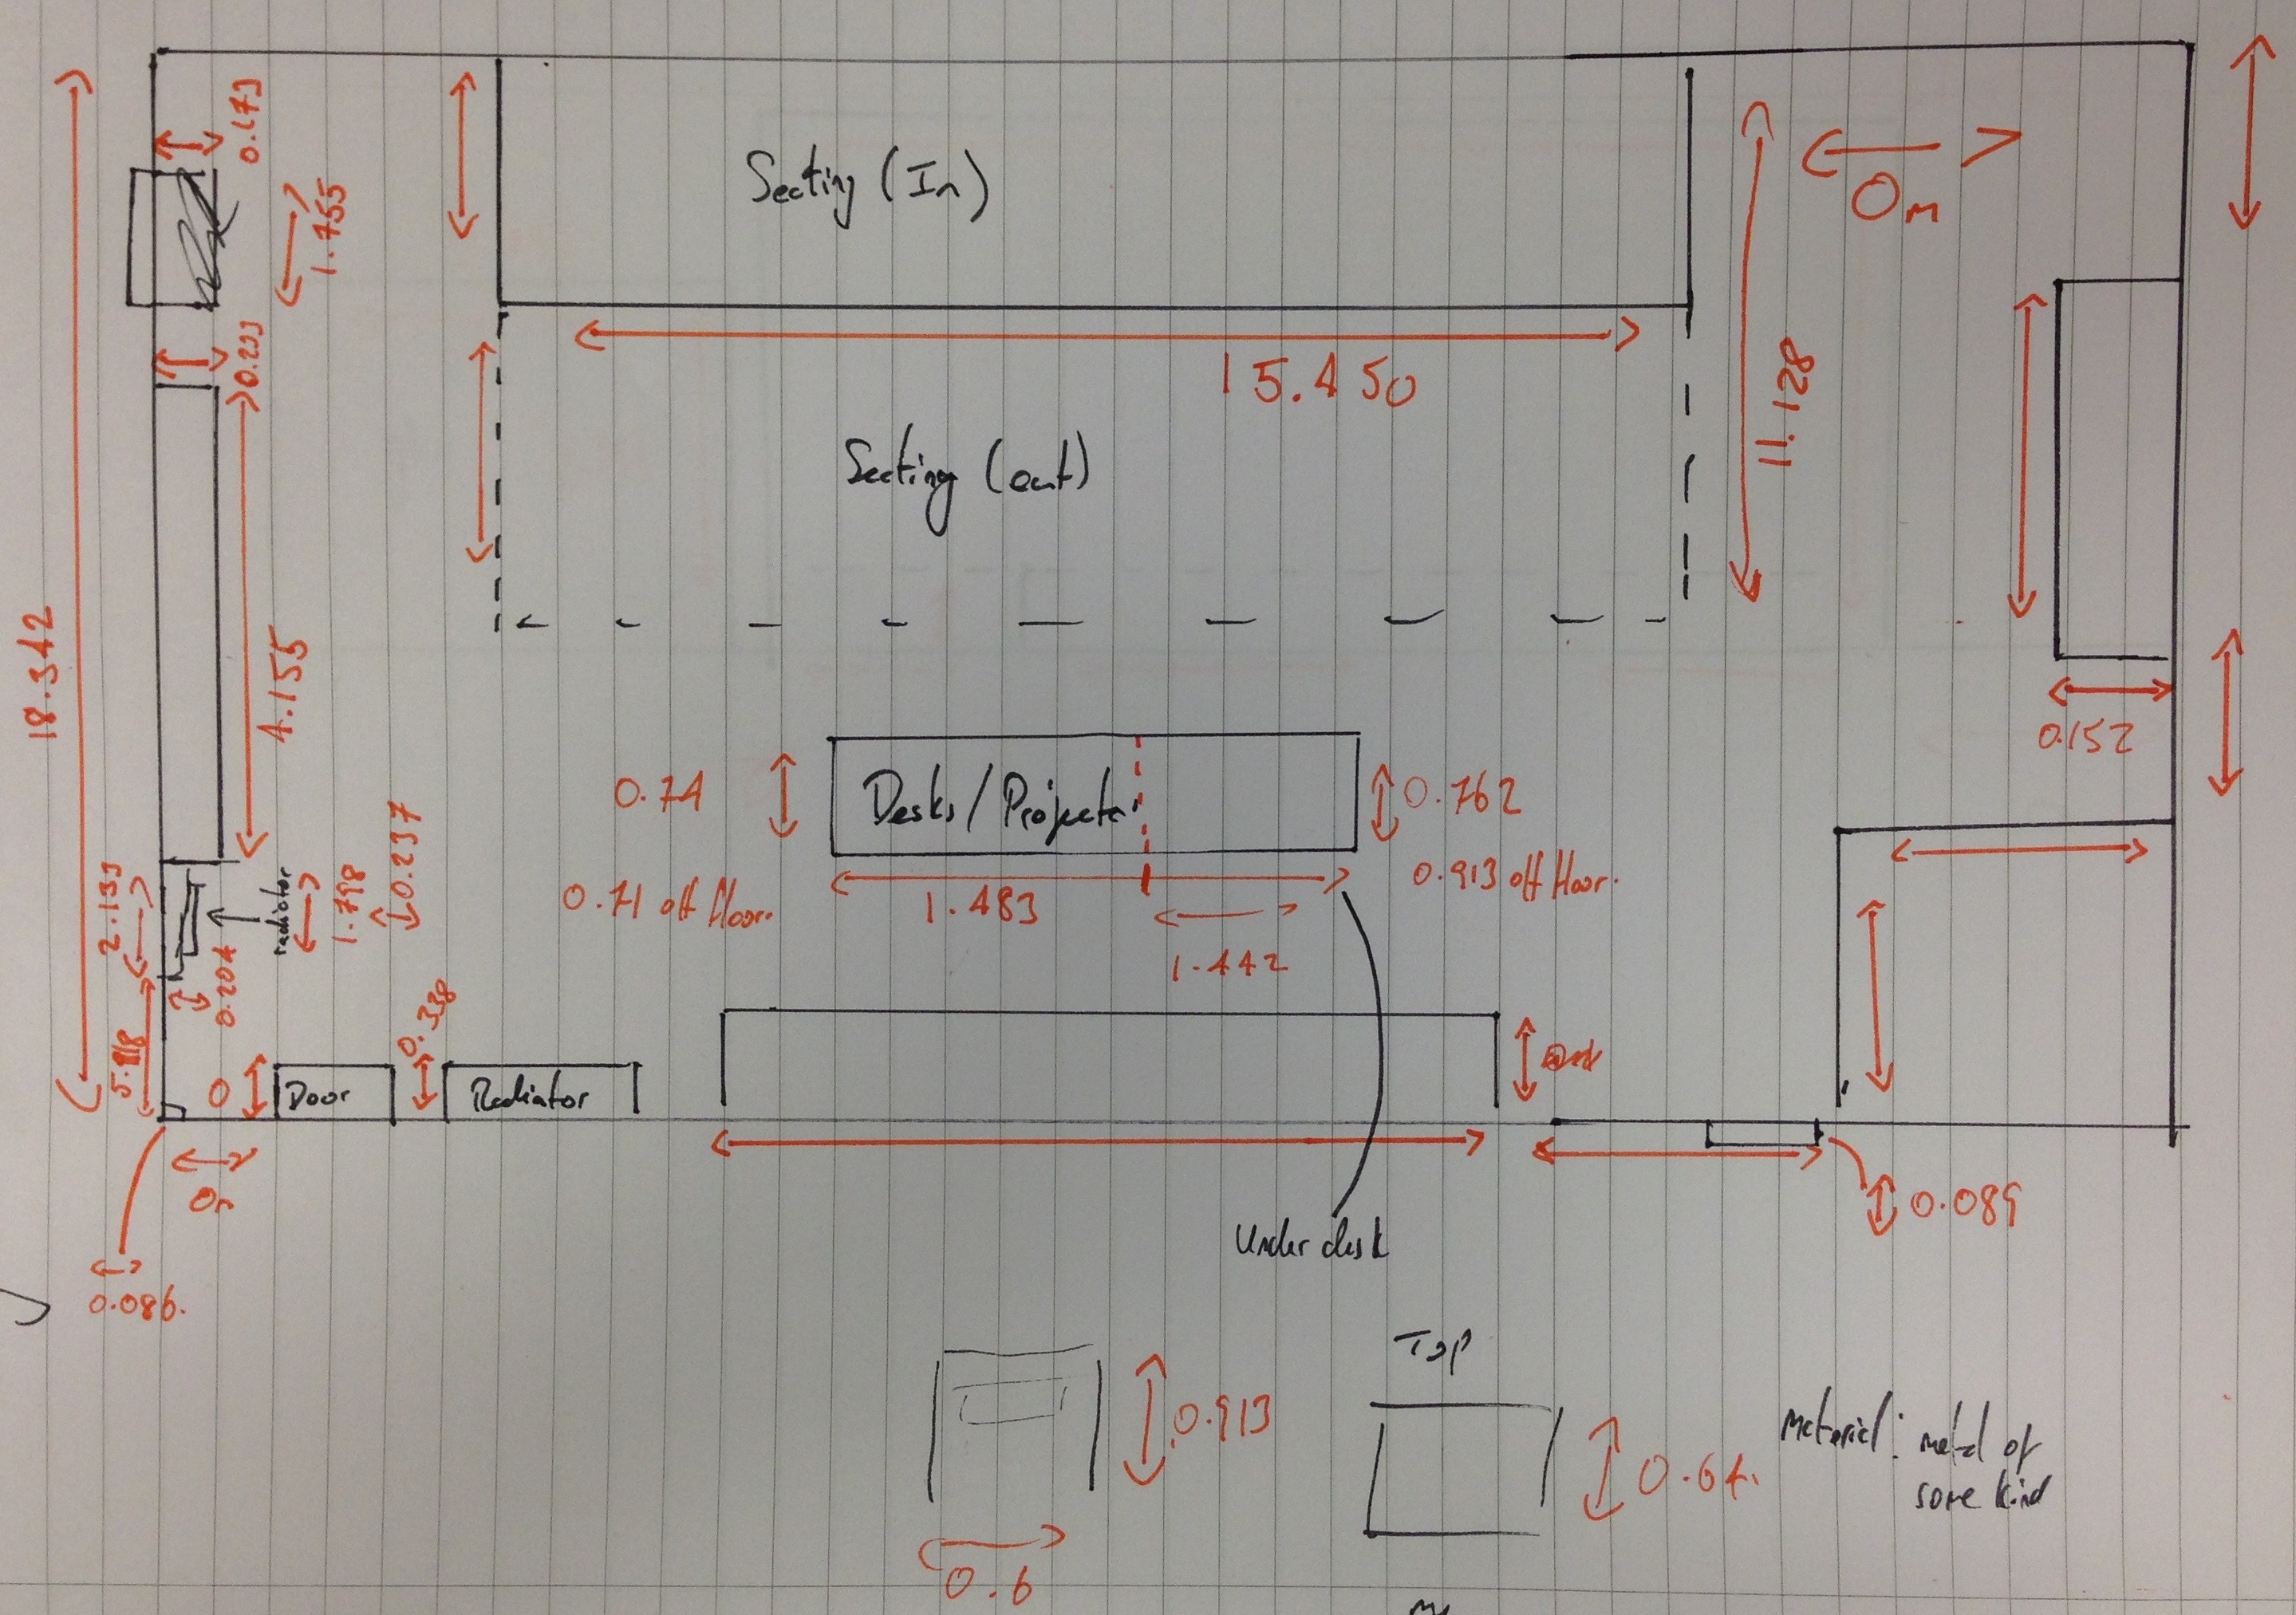
\includegraphics[scale = 0.1]{Sections/Appendix/AppendixA/images/bluePrintTop.jpg}
			\caption{Annotated blueprint of Hendrix Hall from a birds-eye view}
			\label{blueprintTop}
		\end{figure}

		%-------------Real Vs Sku Images-------------%
		\begin{figure}[H]
				\centerline{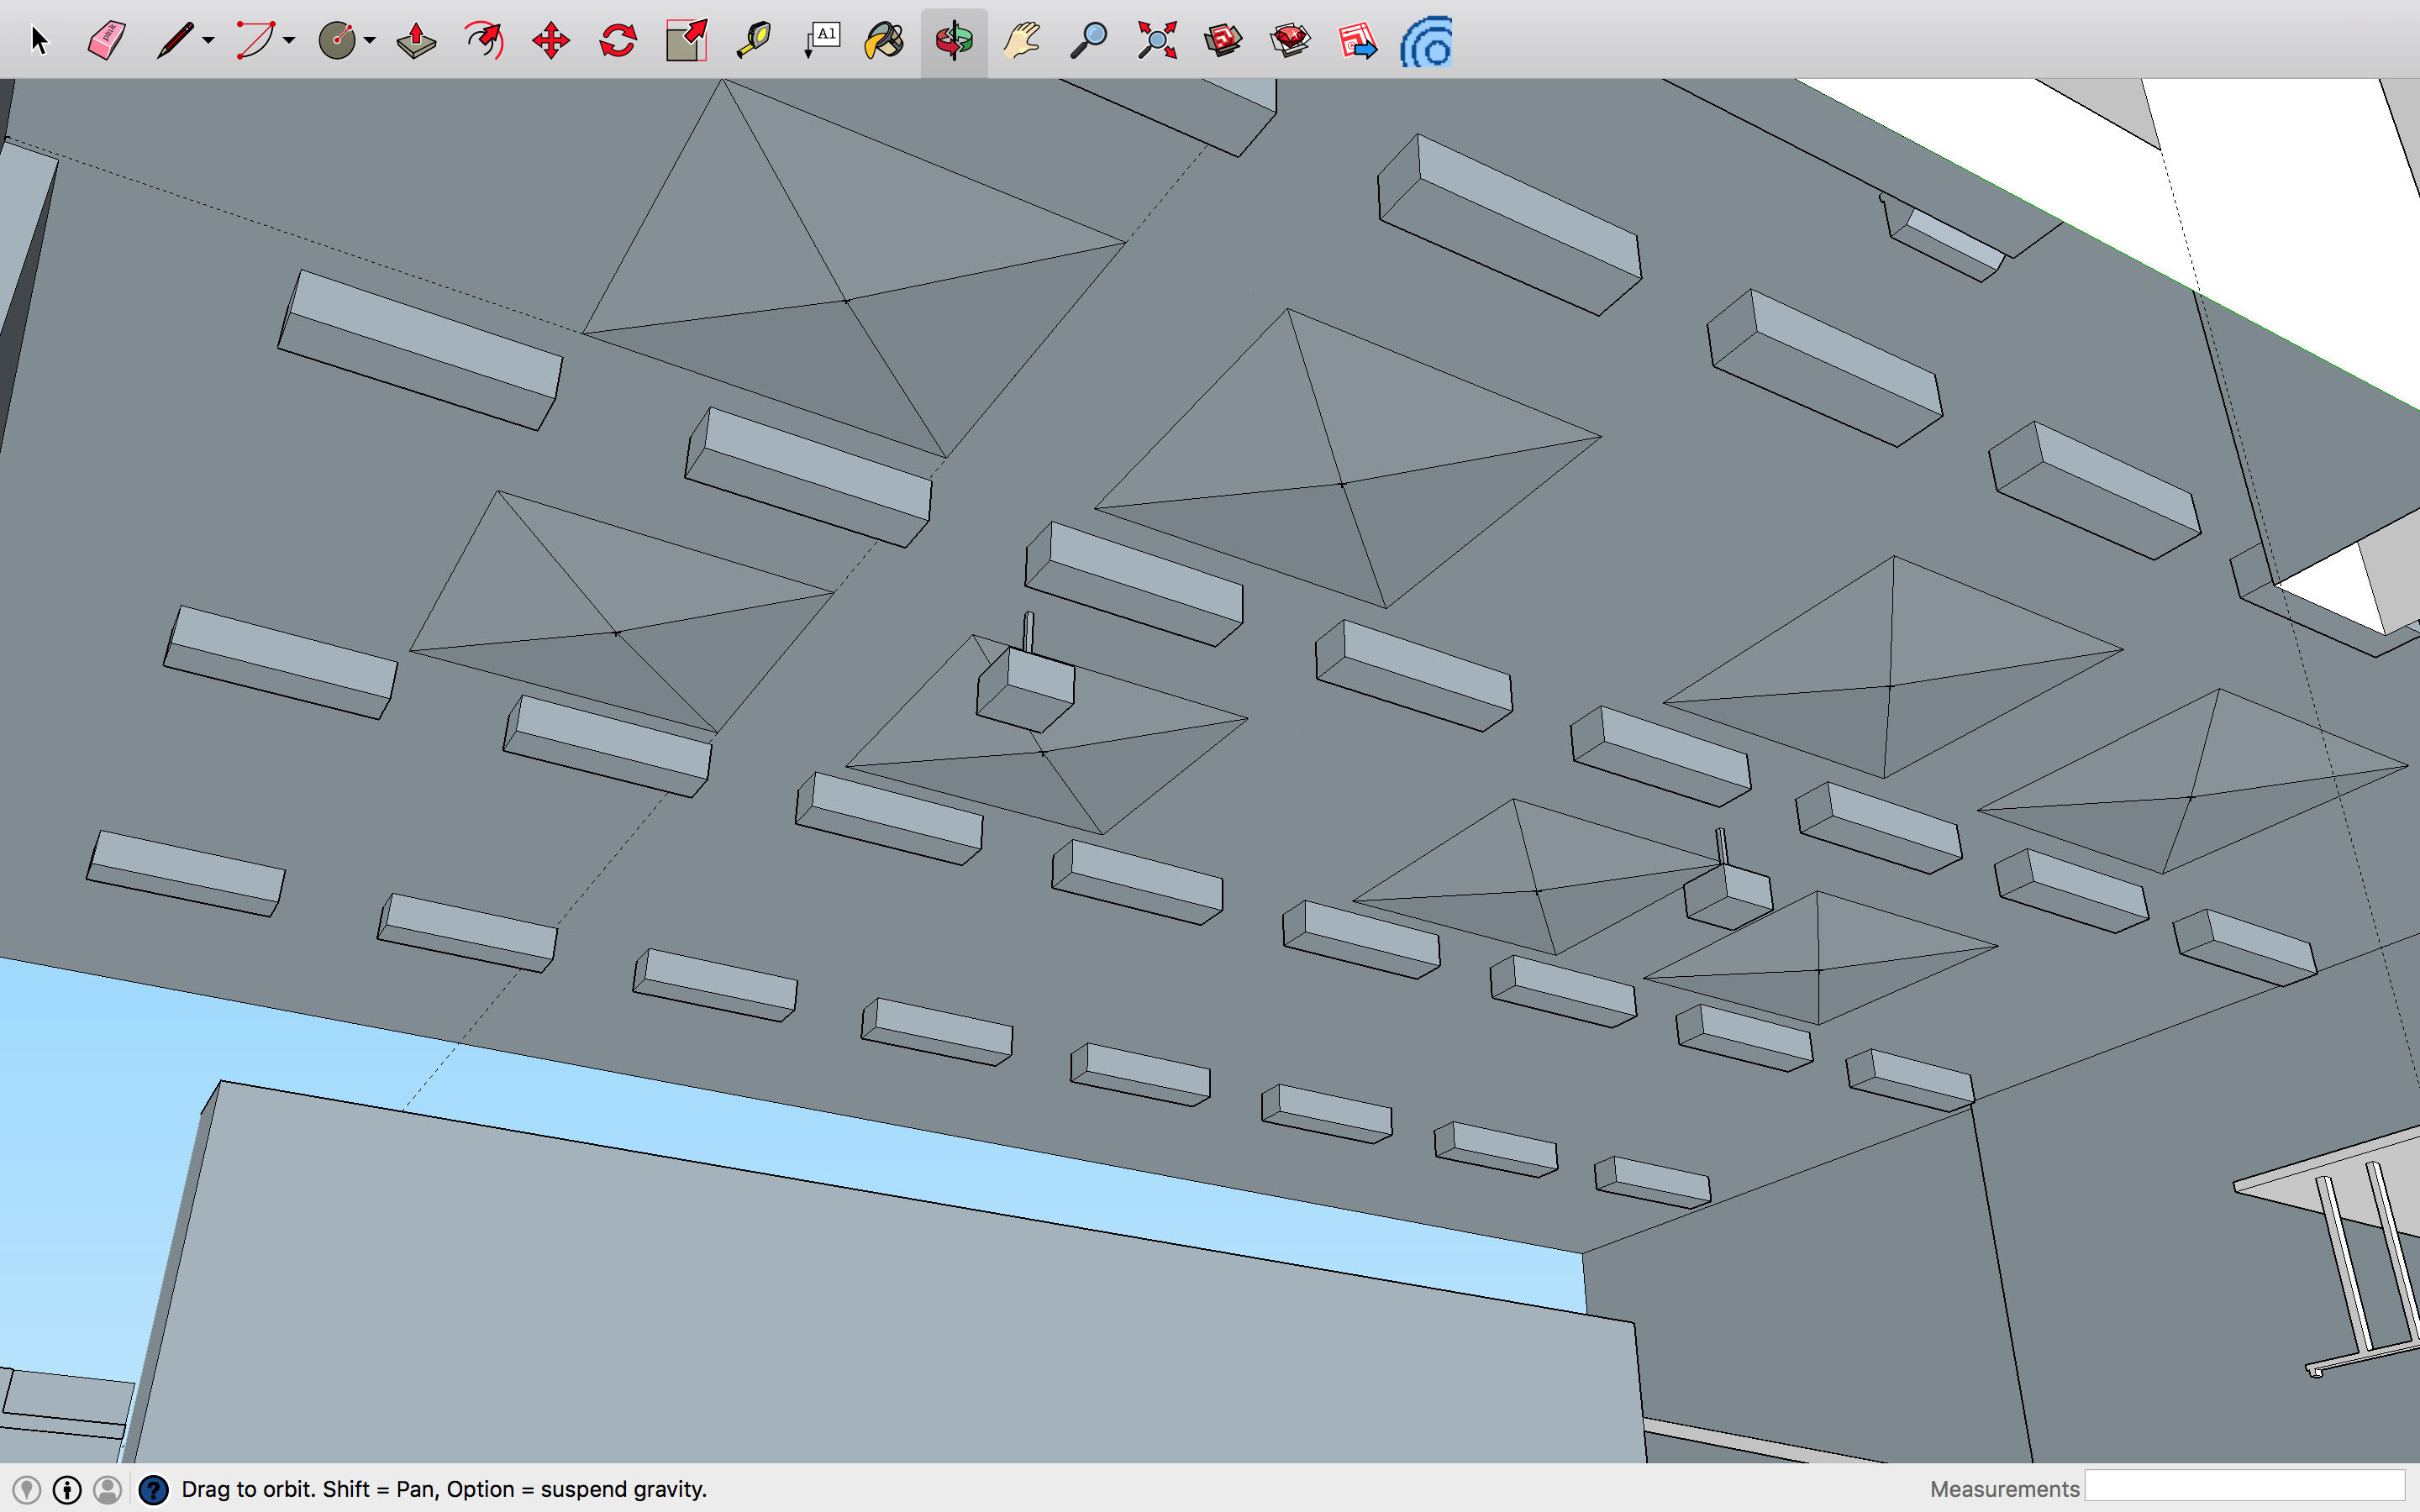
\includegraphics[scale = 0.2]{Sections/Appendix/AppendixA/images/realVsSku/roofSku.png}}
				\centerline{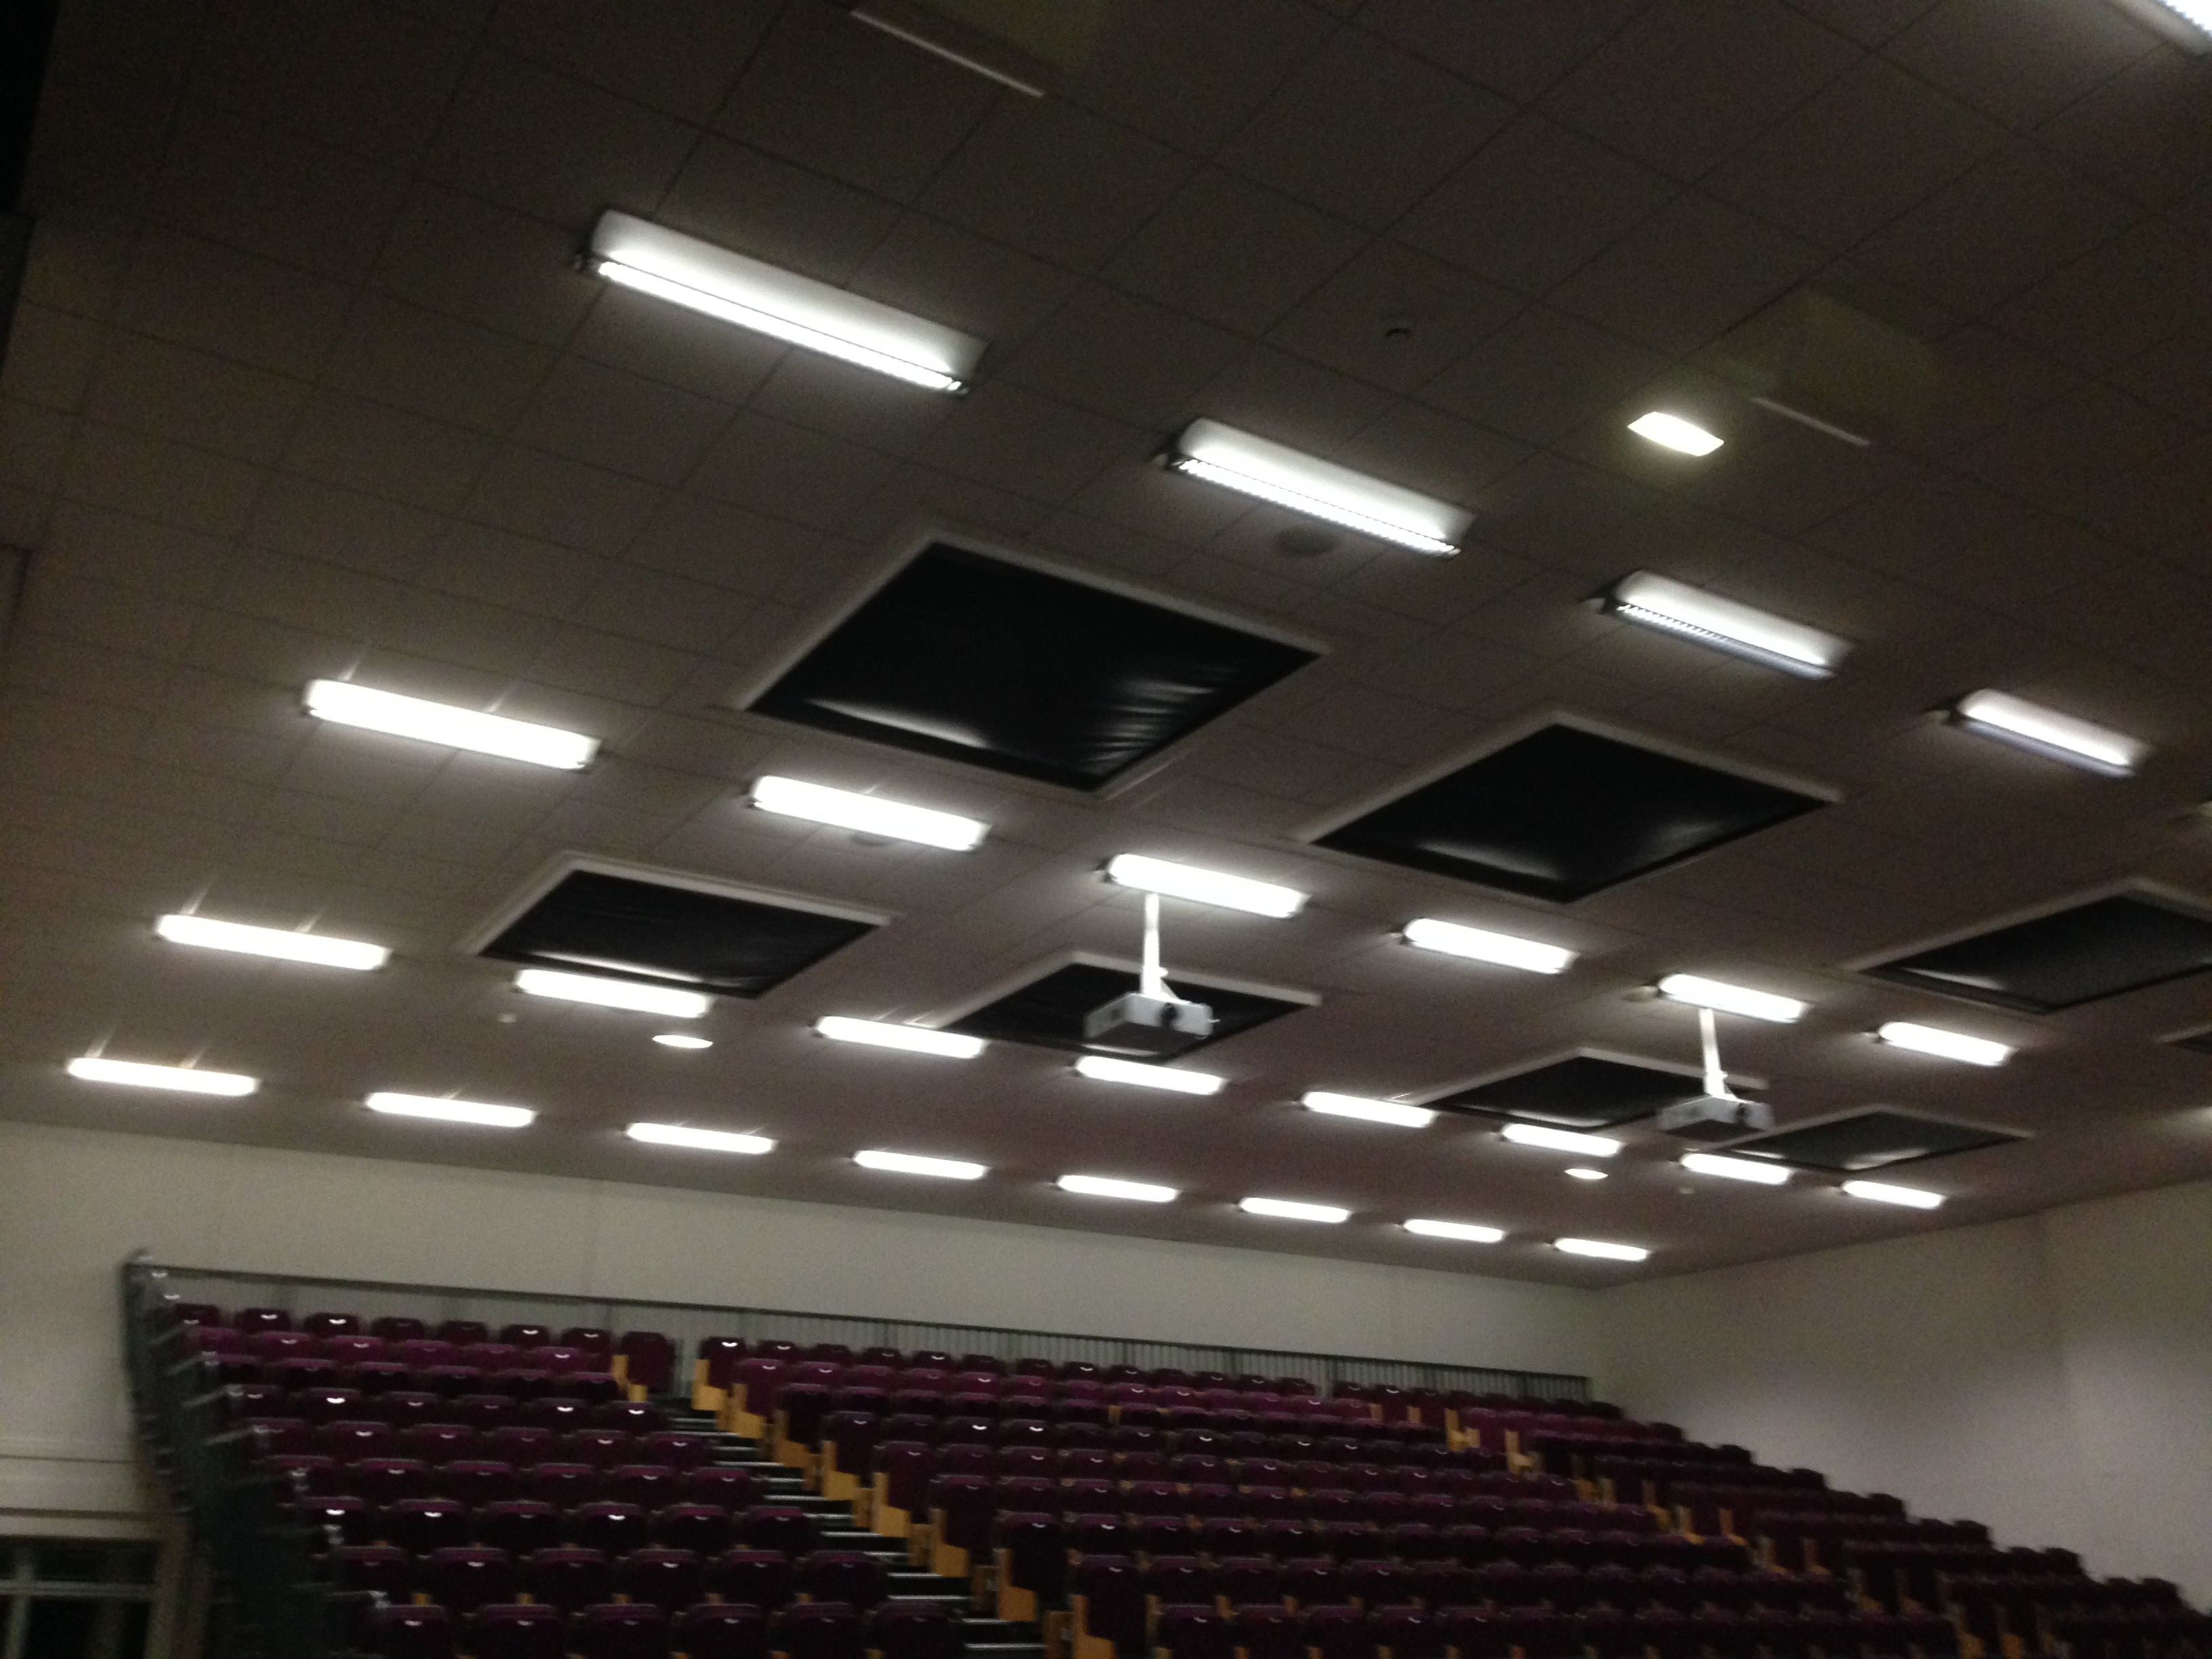
\includegraphics[scale = 0.1]{Sections/Appendix/AppendixA/images/realVsSku/roofReal.jpg}}
			\caption{Real Vs SKU Roof}
		\end{figure}

		\begin{figure}[H]
				\centerline{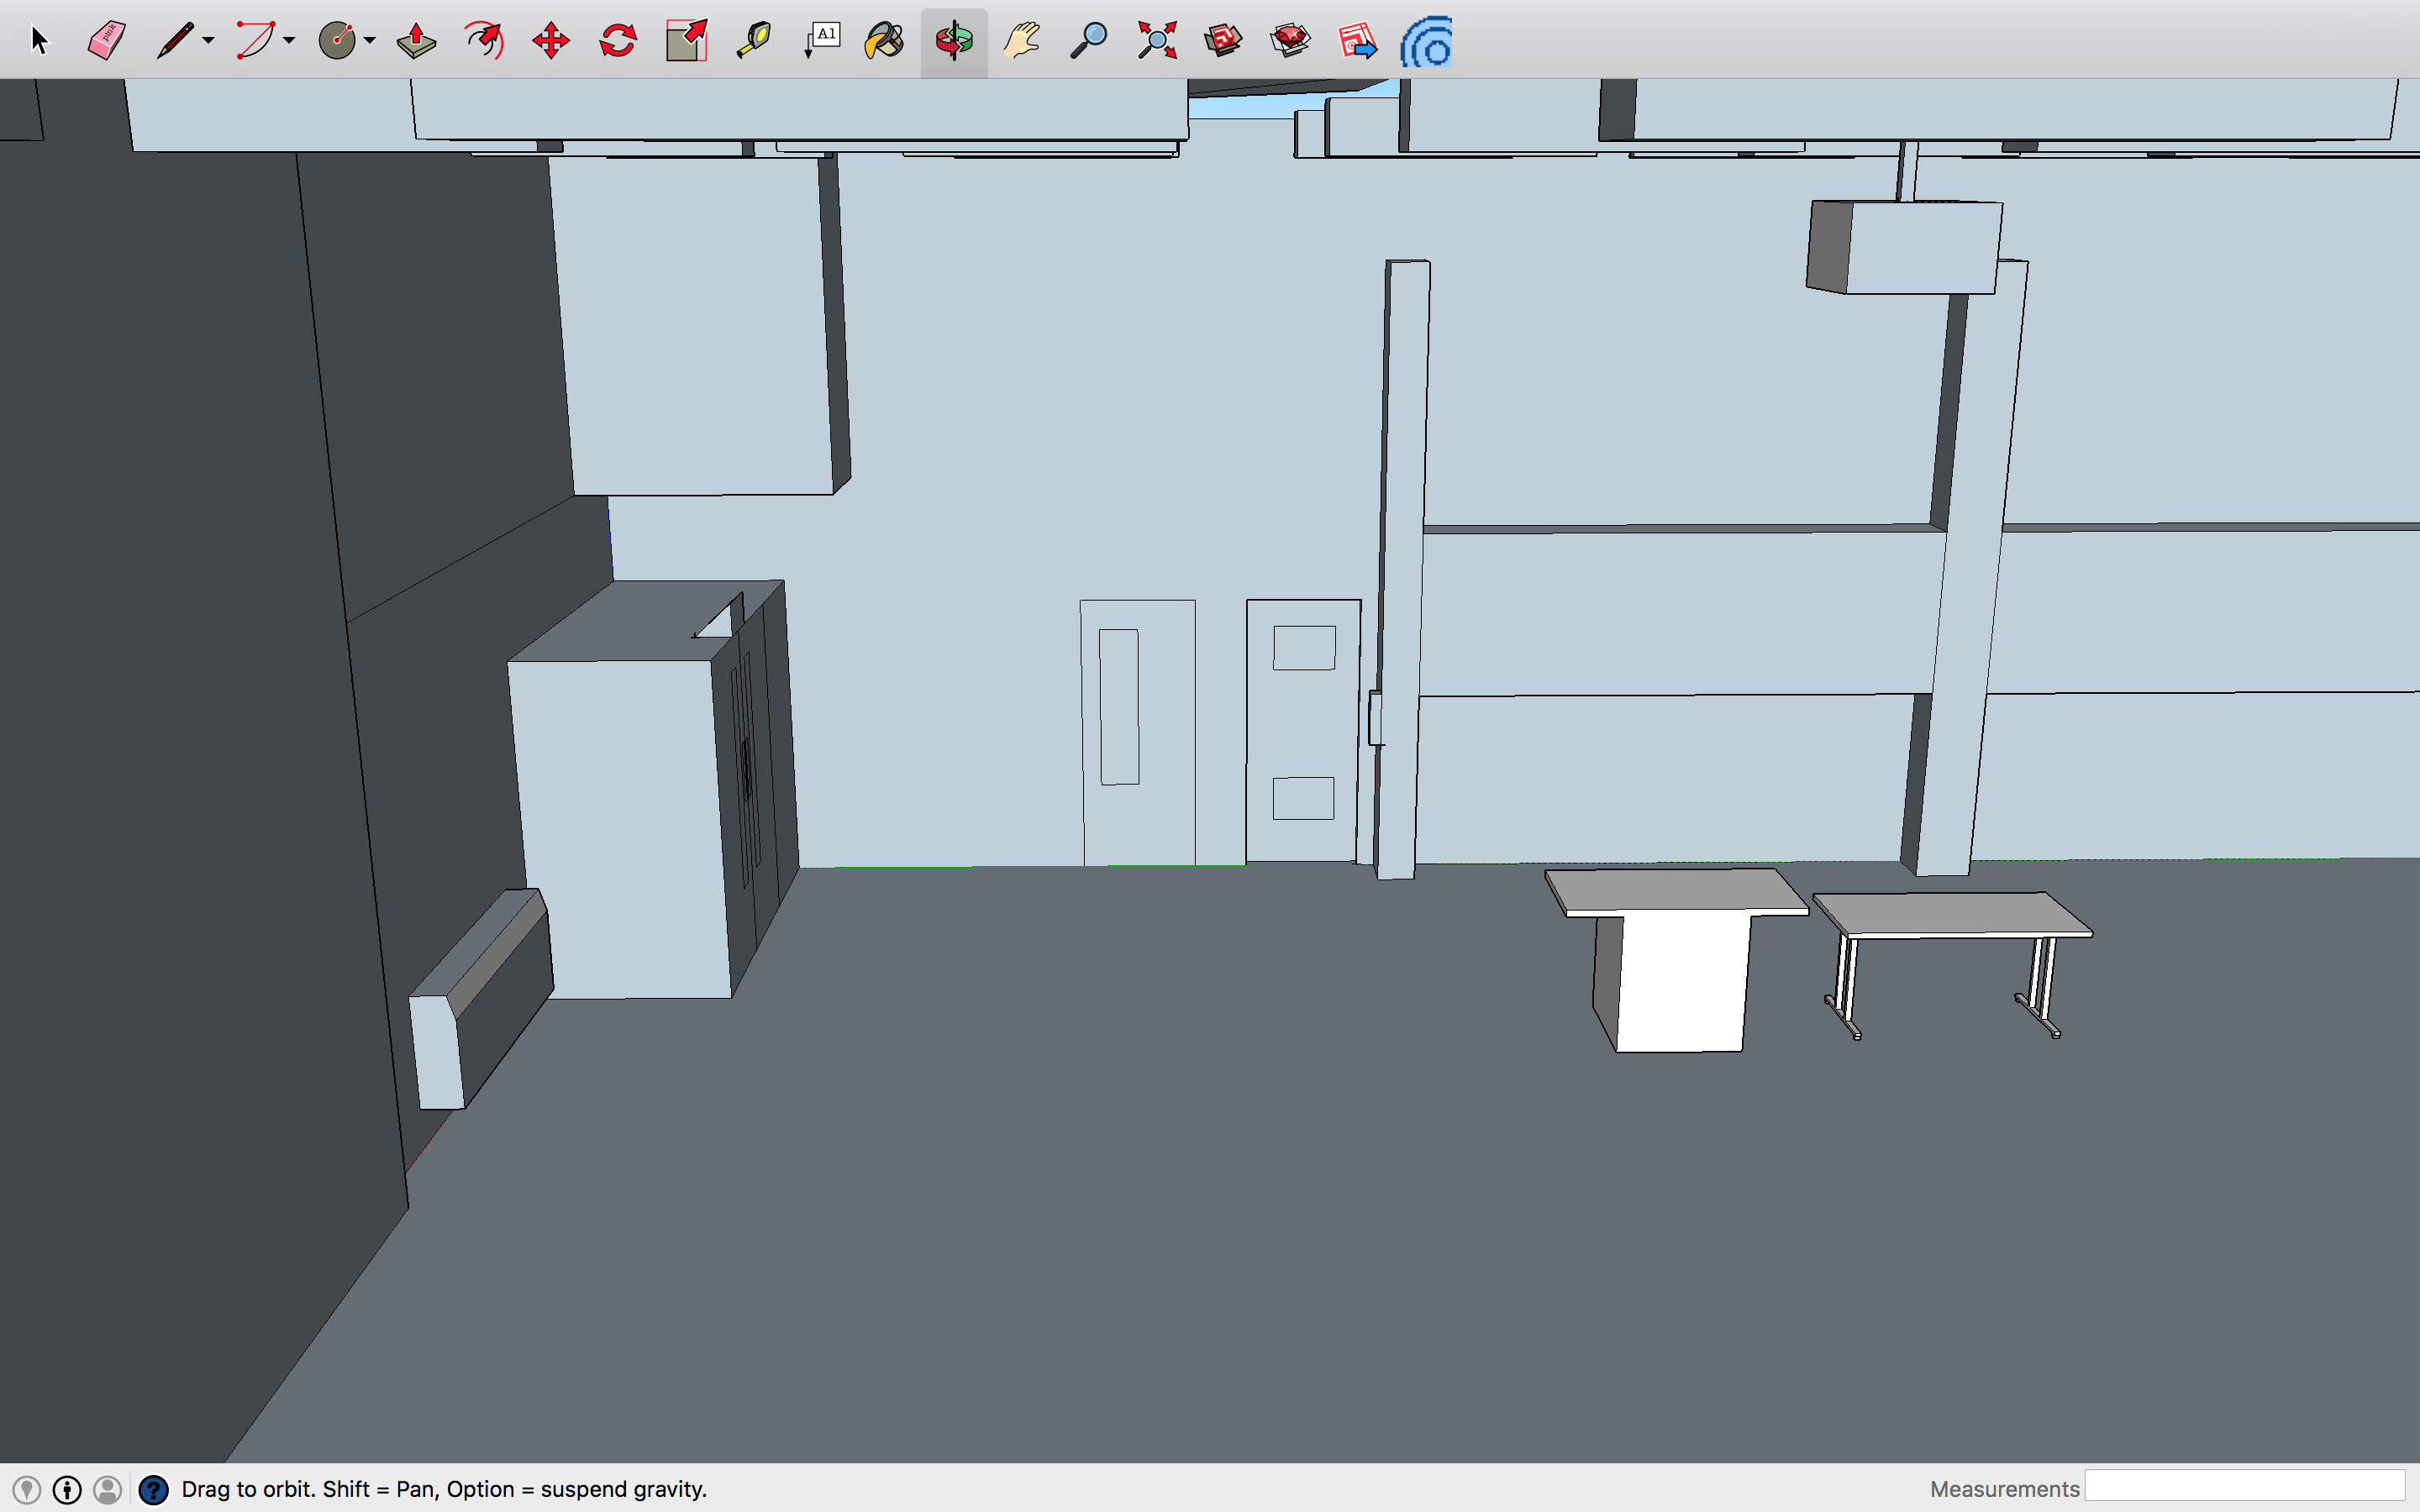
\includegraphics[scale = 0.2]{Sections/Appendix/AppendixA/images/realVsSku/fromSeatsSku.png}}
				\centerline{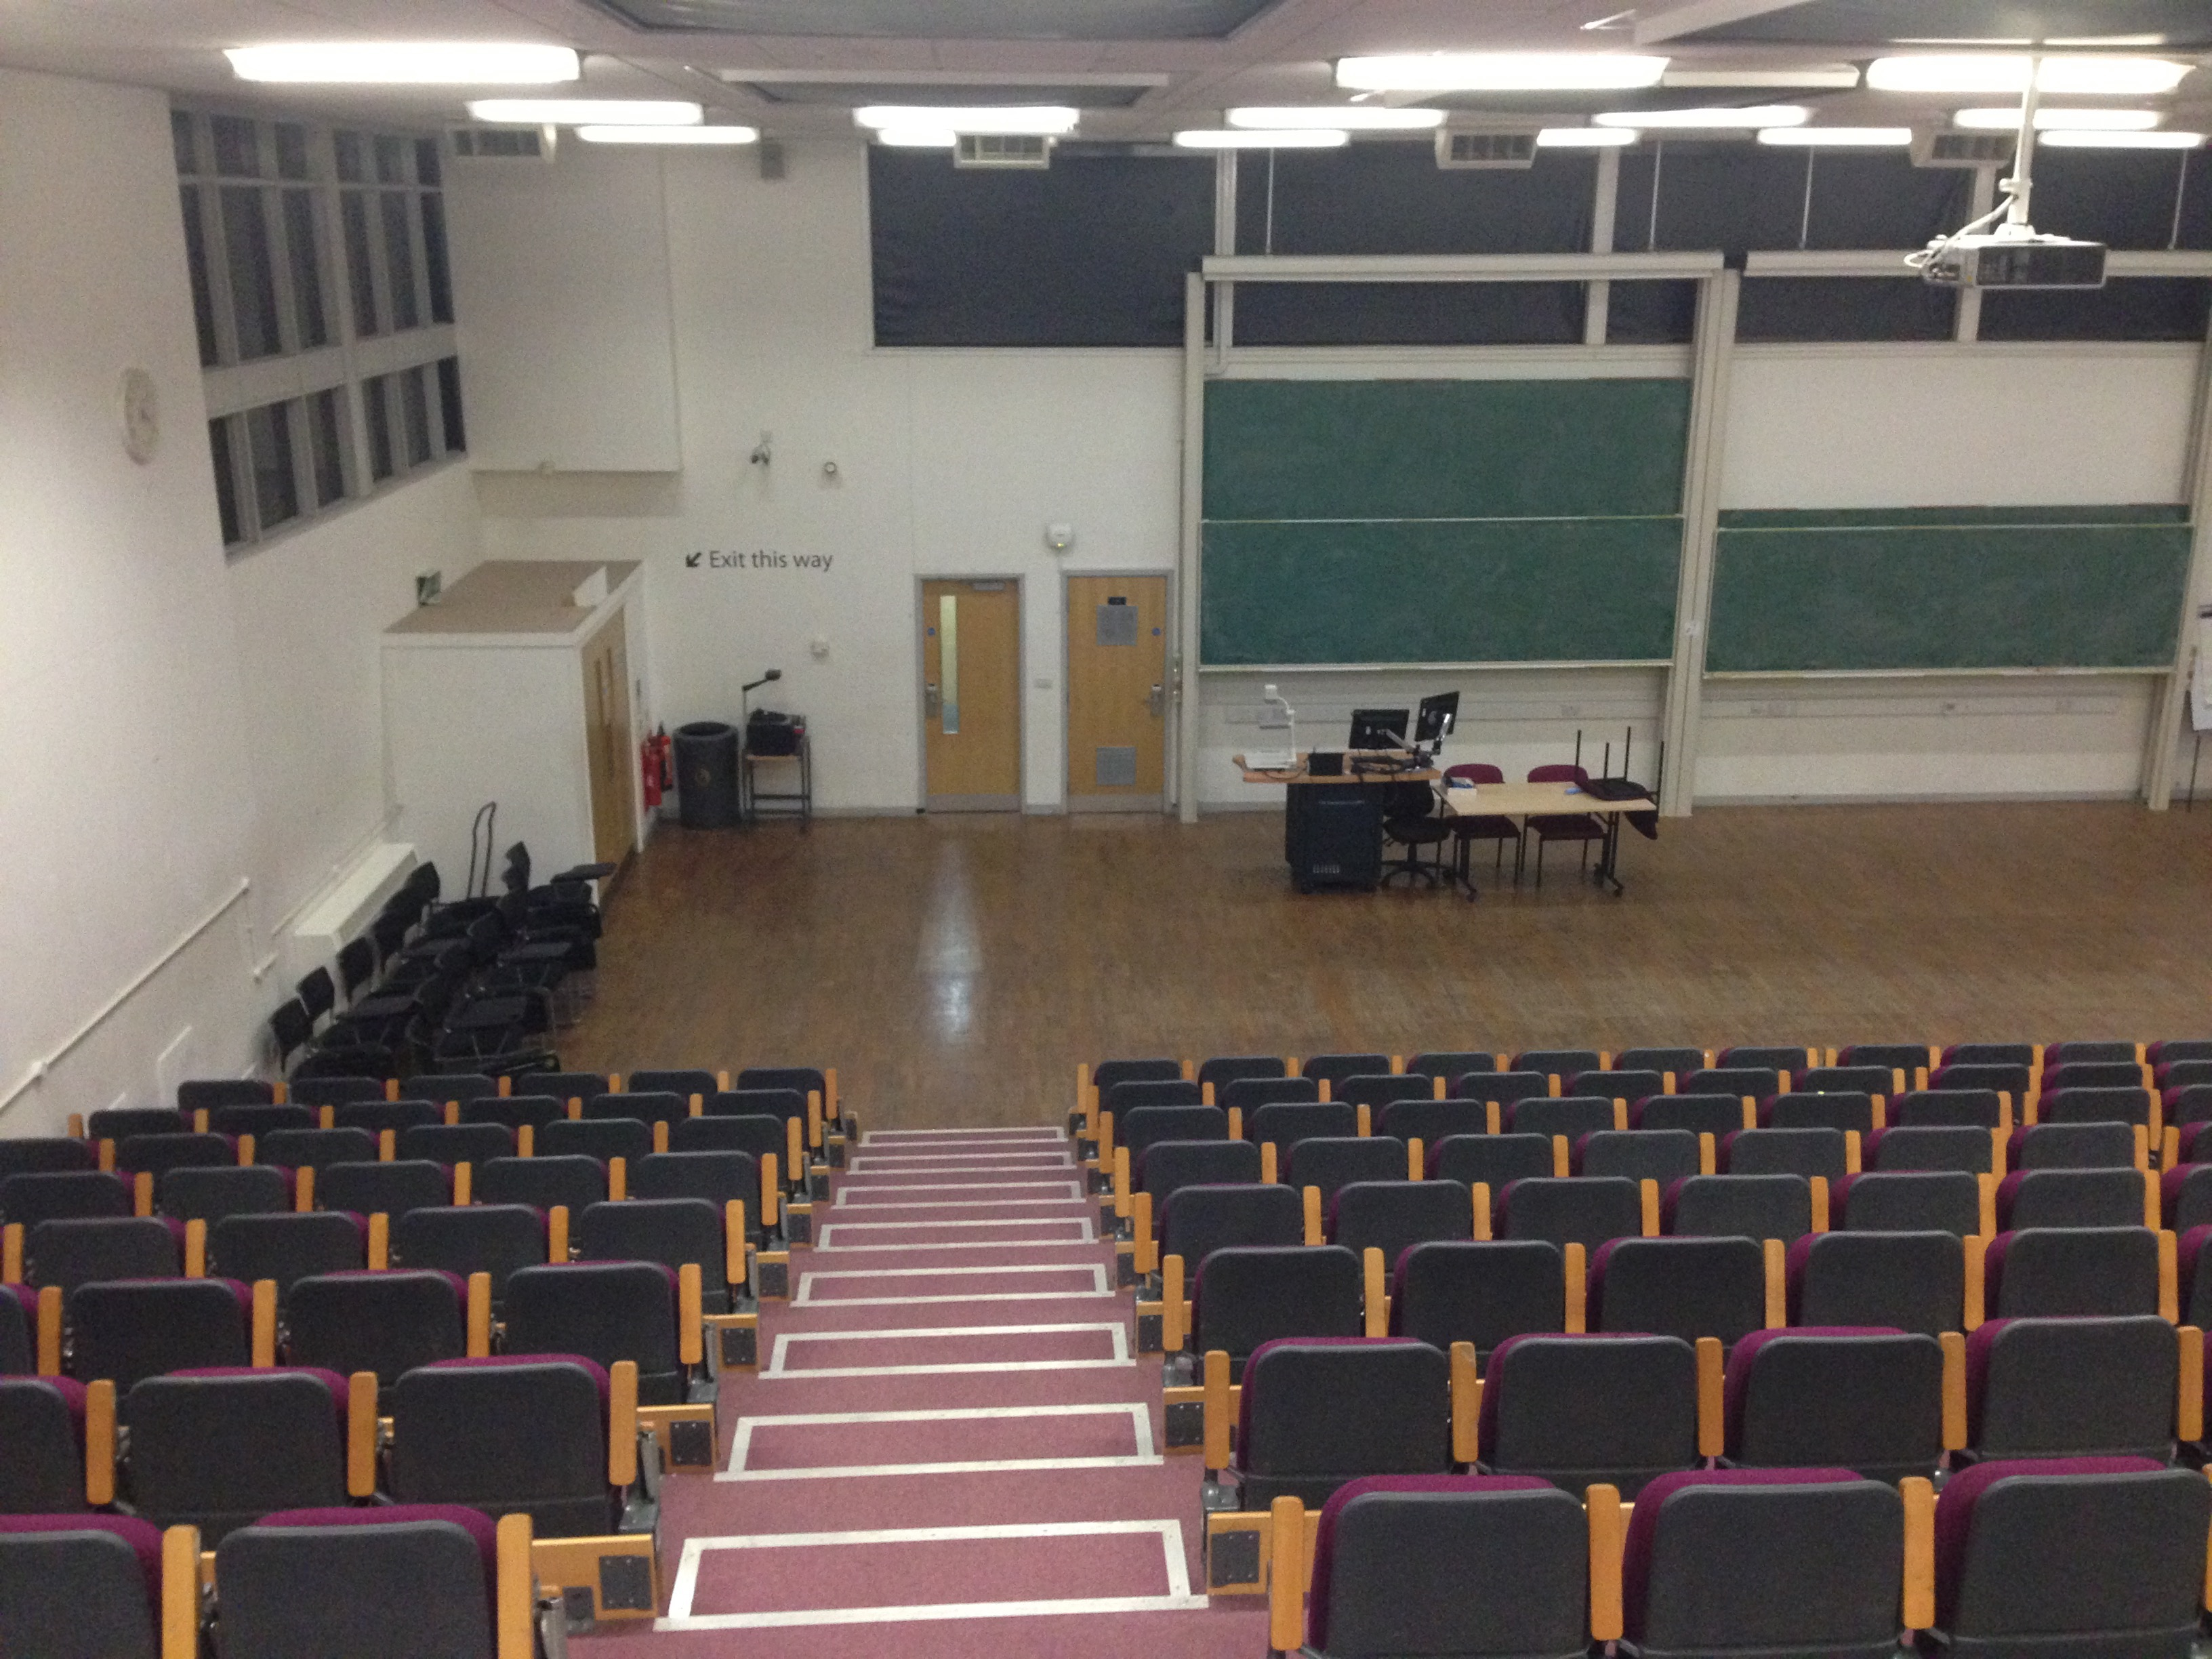
\includegraphics[scale = 0.1]{Sections/Appendix/AppendixA/images/realVsSku/fromSeatsReal.jpg}}
			\caption{Real Vs SKU Roof}
		\end{figure}

		\begin{figure}[H]
				\centerline{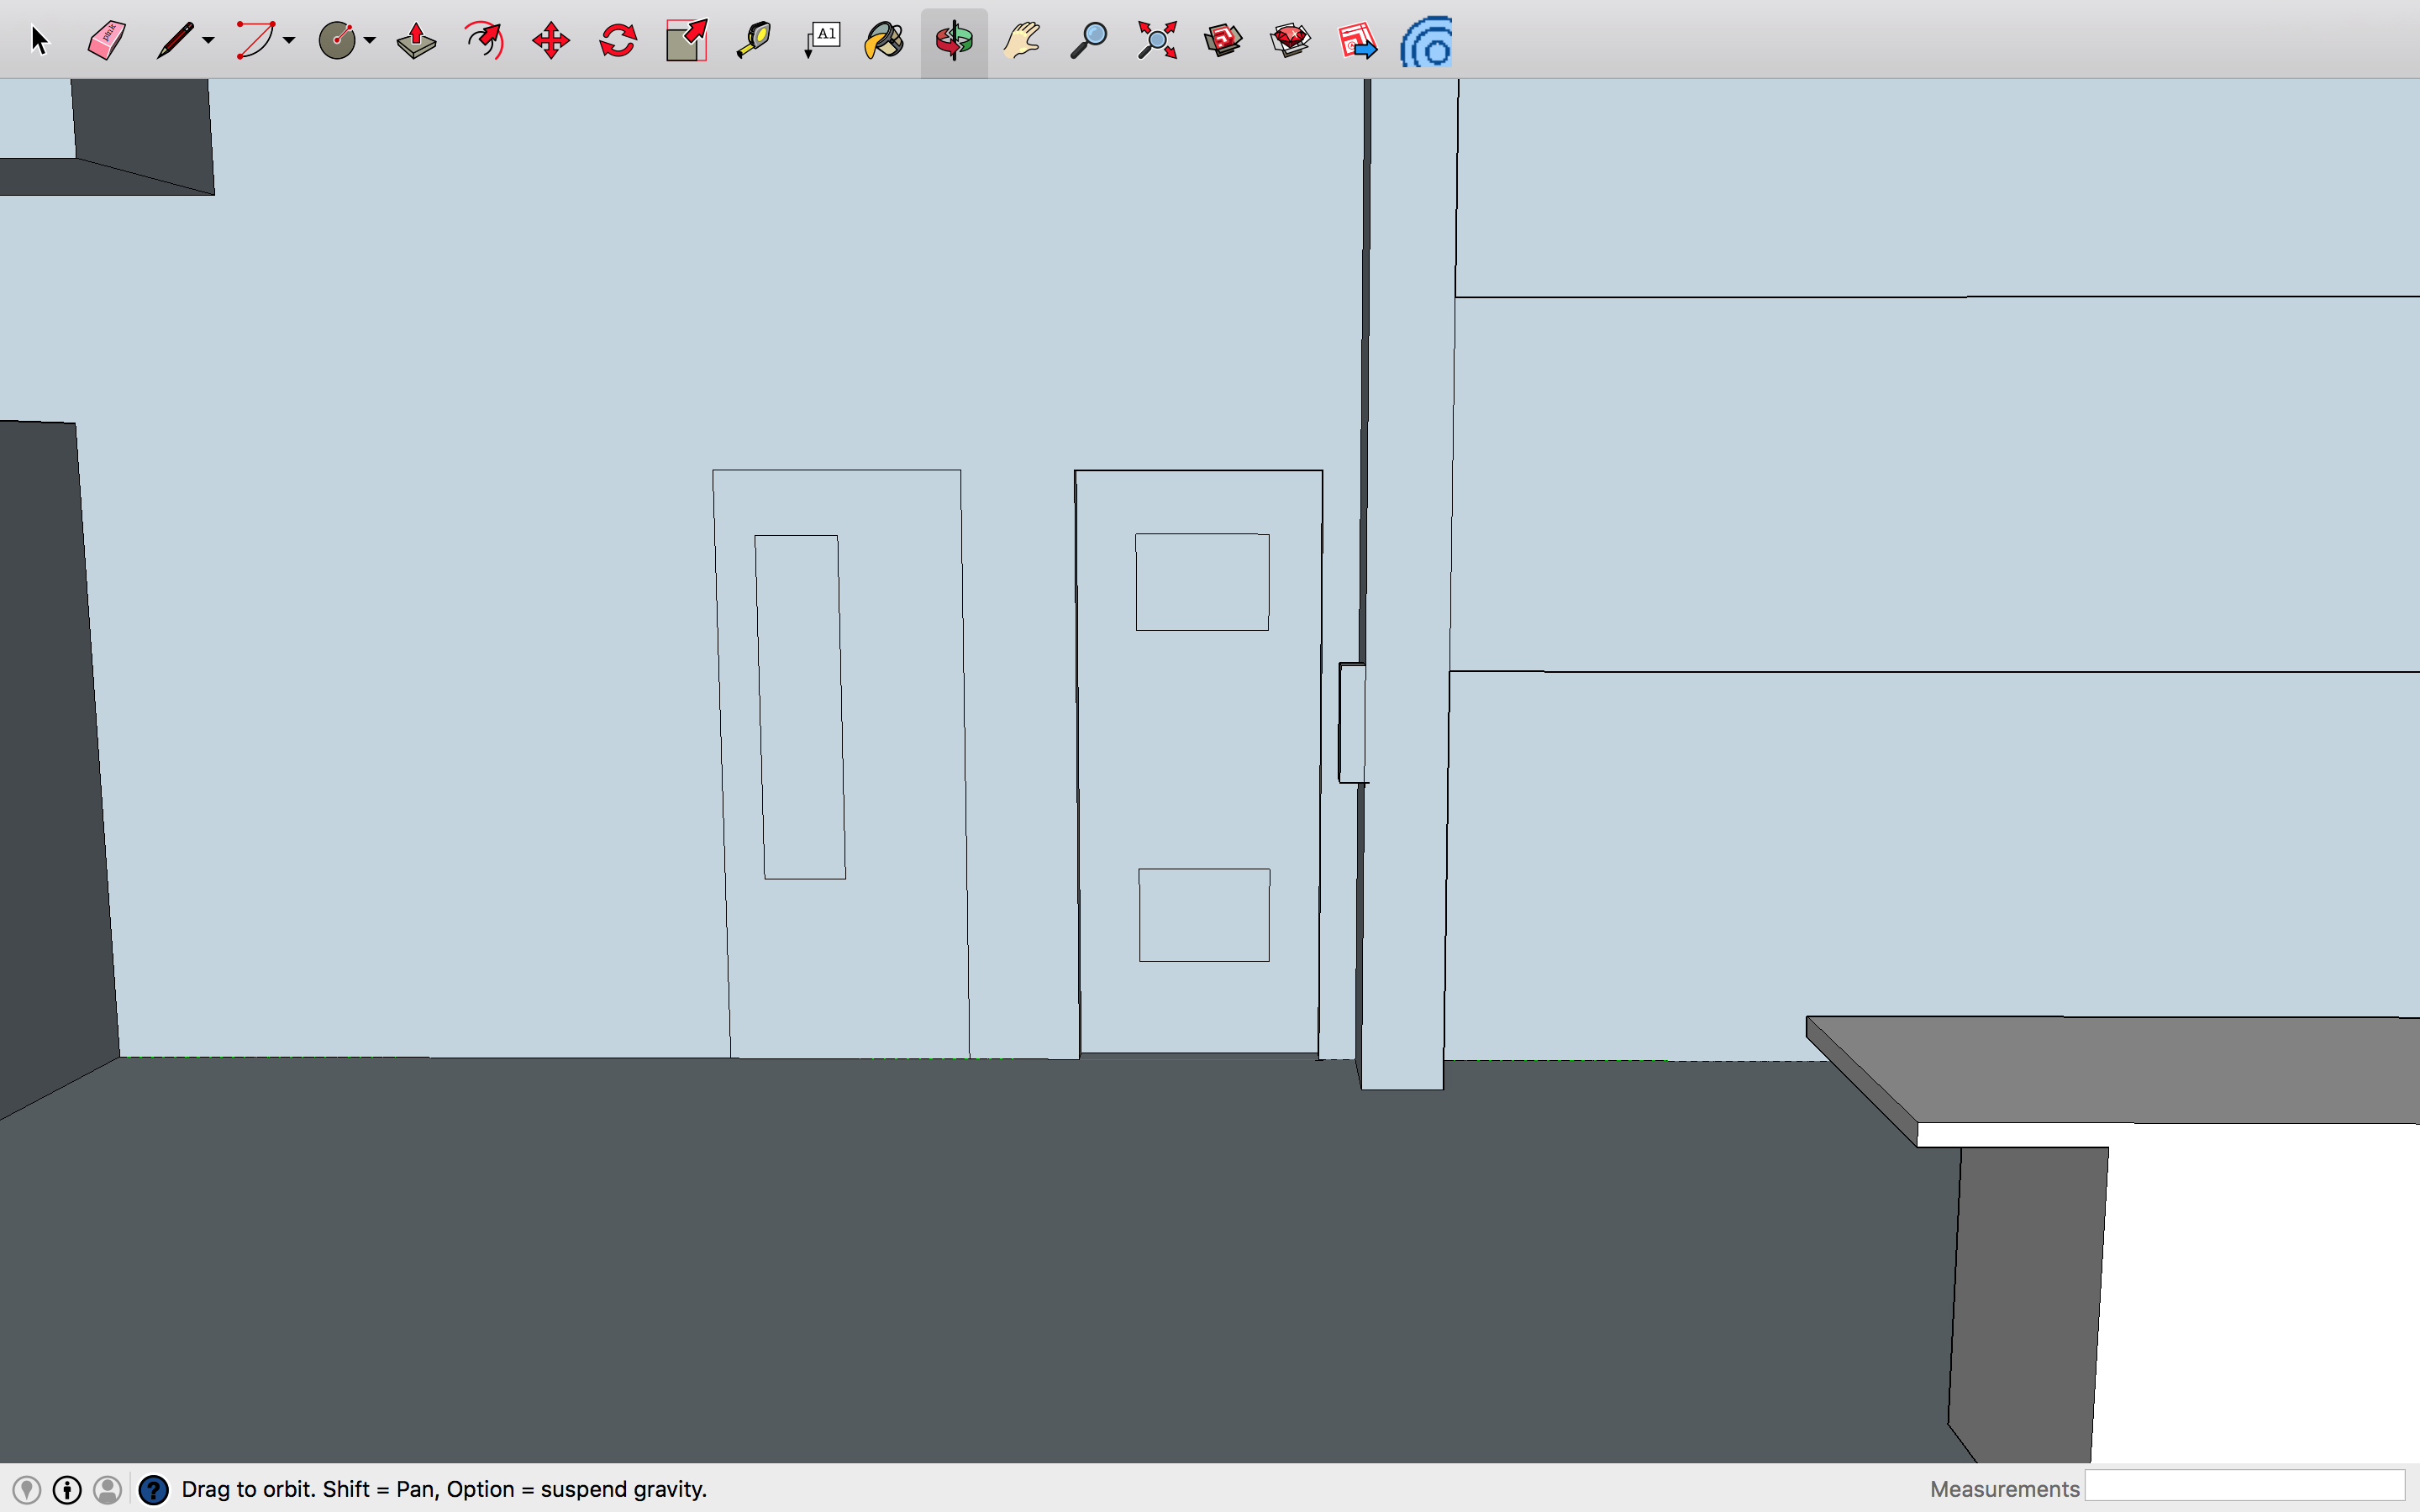
\includegraphics[scale = 0.2]{Sections/Appendix/AppendixA/images/realVsSku/doorsSku.png}}
				\centerline{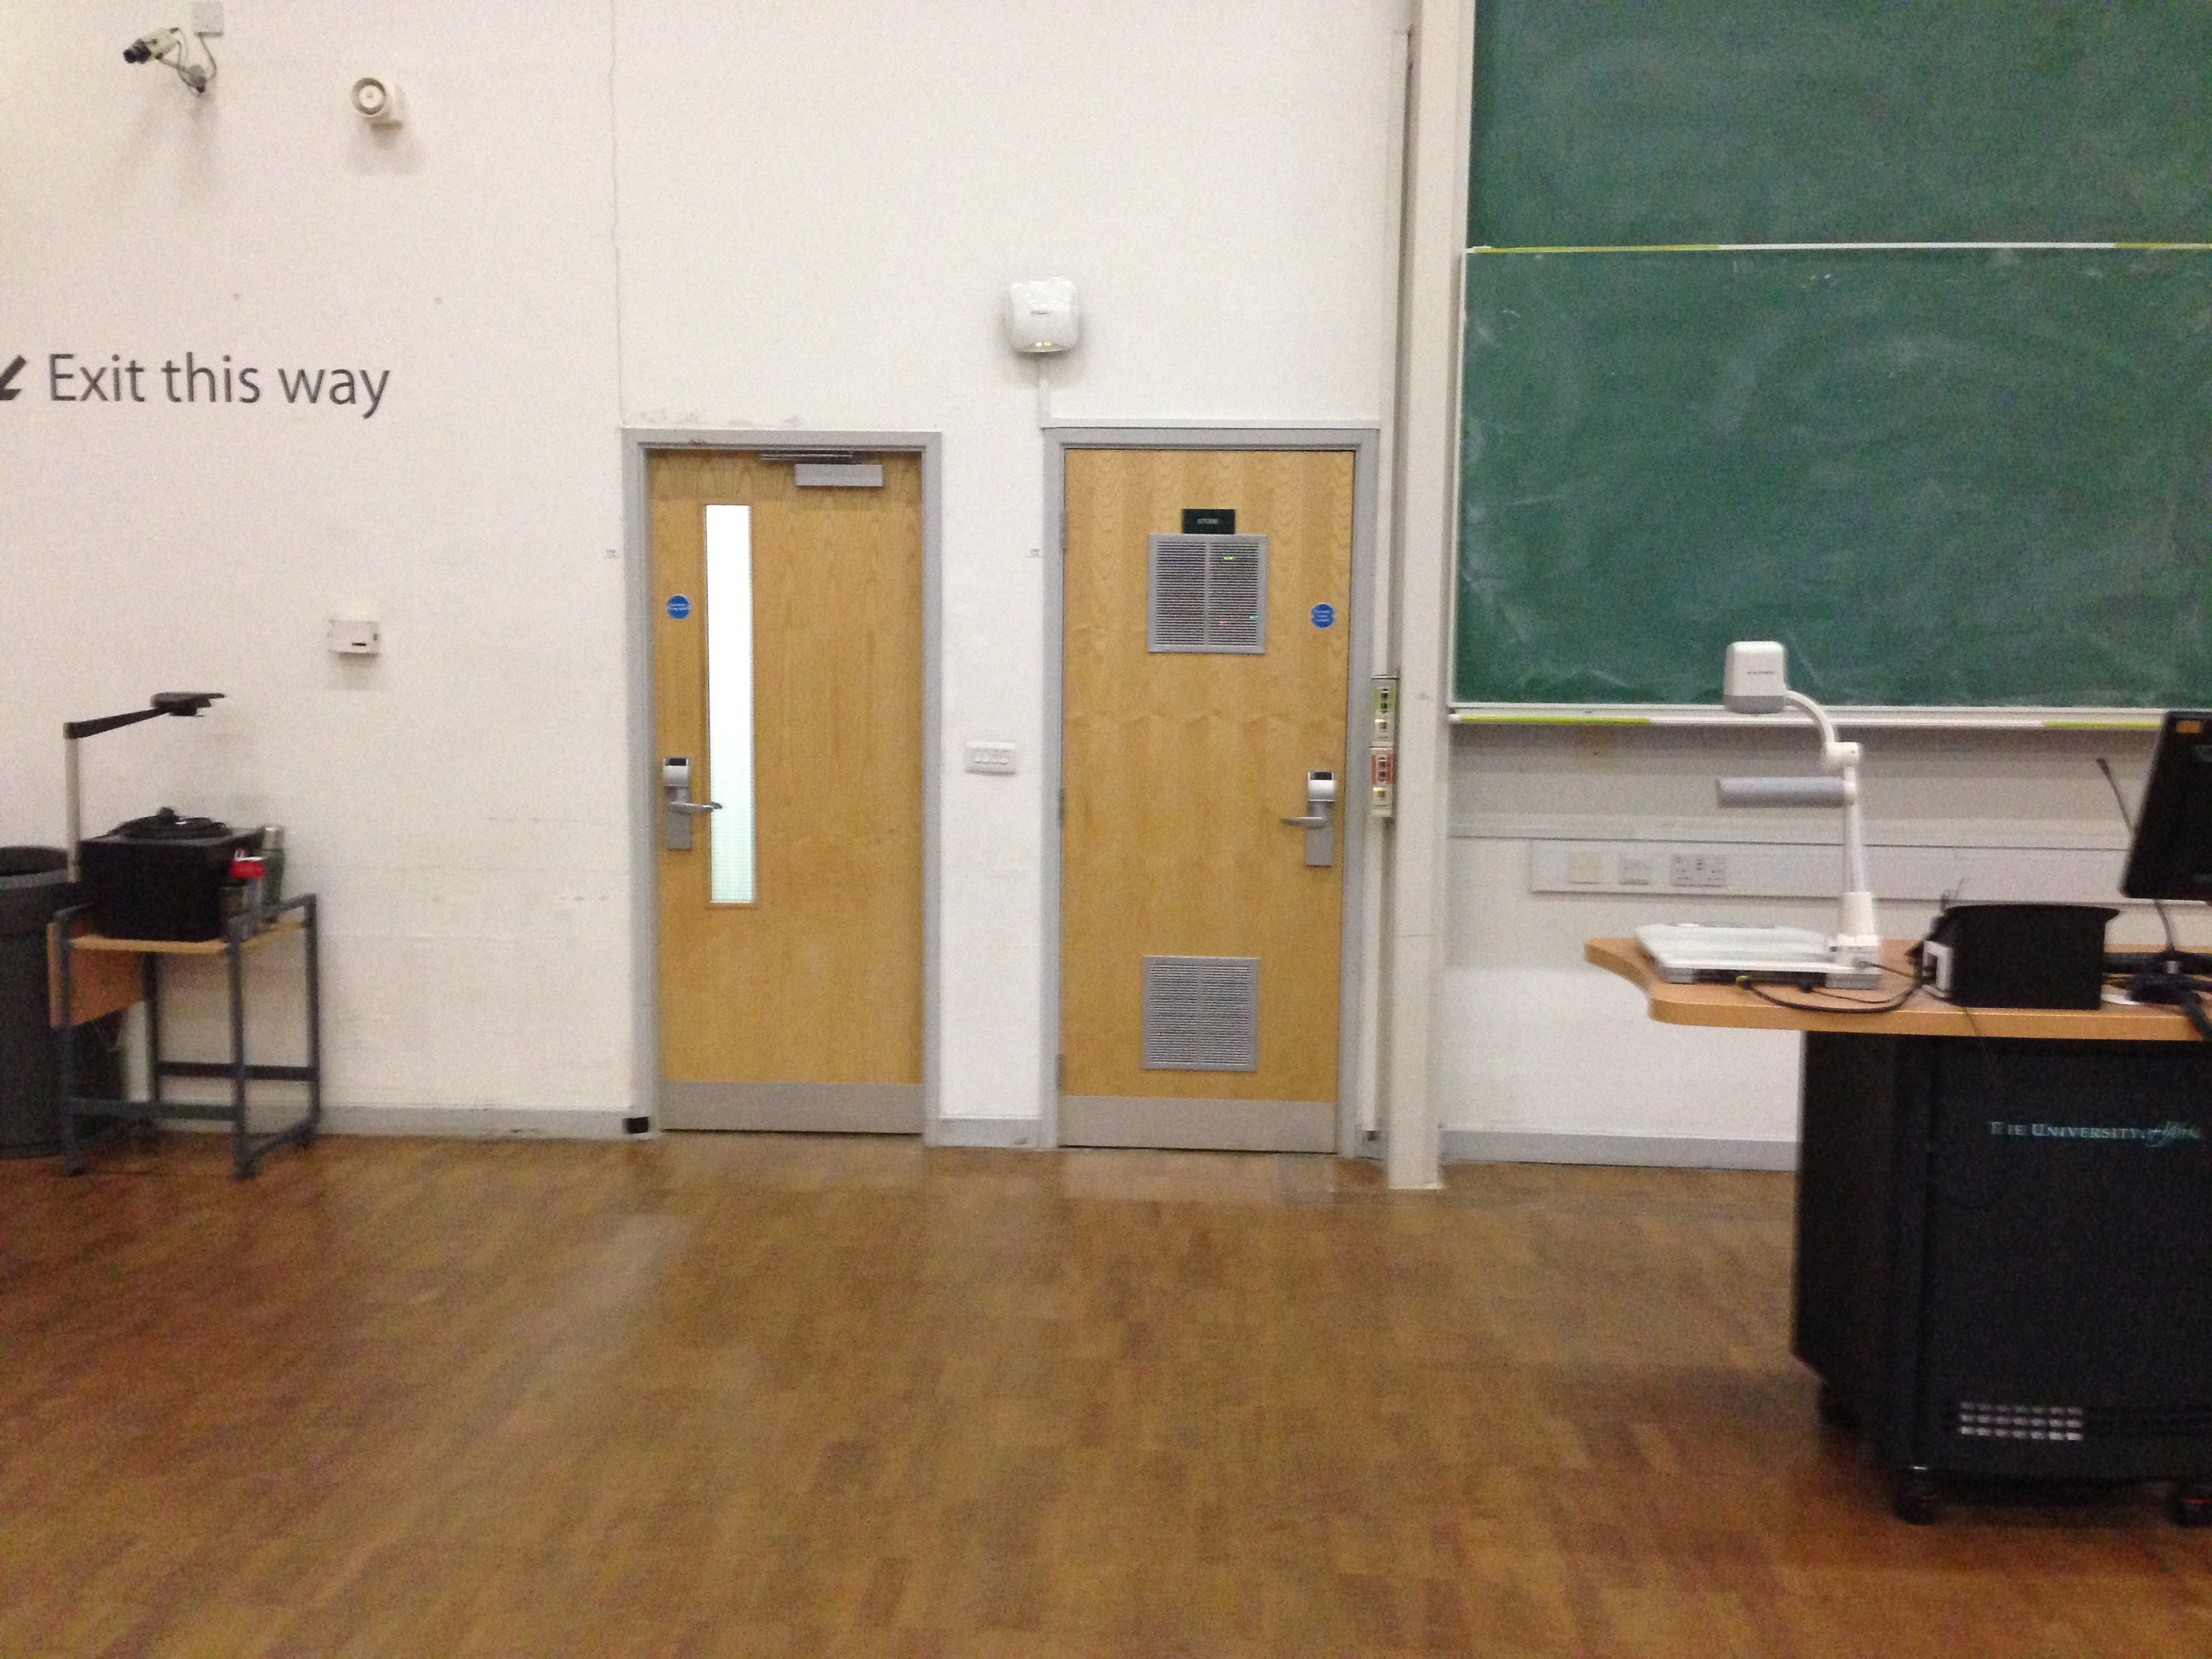
\includegraphics[scale = 0.1]{Sections/Appendix/AppendixA/images/realVsSku/doorsReal.jpg}}
			\caption{Real Vs SKU Roof}
		\end{figure}

	%-------------ODEON APPENDIX-------------%
	\section{Appendix B}
	\label{appendixB}

		%-------------RIR GRIDS-------------%
		\begin{minipage}{0.5\textwidth}
		\begin{figure}[H]
				\centerline{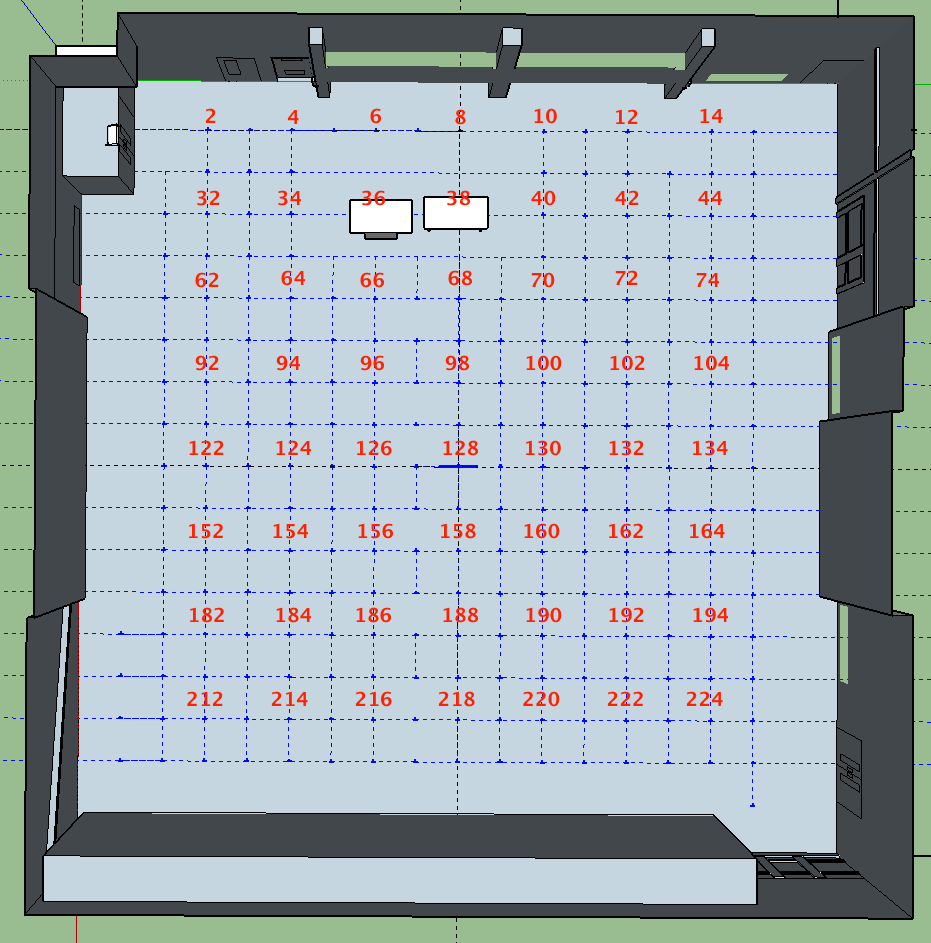
\includegraphics[scale = 0.23]{Sections/Appendix/AppendixA/images/Odeon/2m.png}}
				\caption{\ac{RIR} grid with 2m separation}
				\label{2m}
		\end{figure}
		\end{minipage}
		\begin{minipage}{0.5\textwidth}
		\begin{figure}[H]
				\centerline{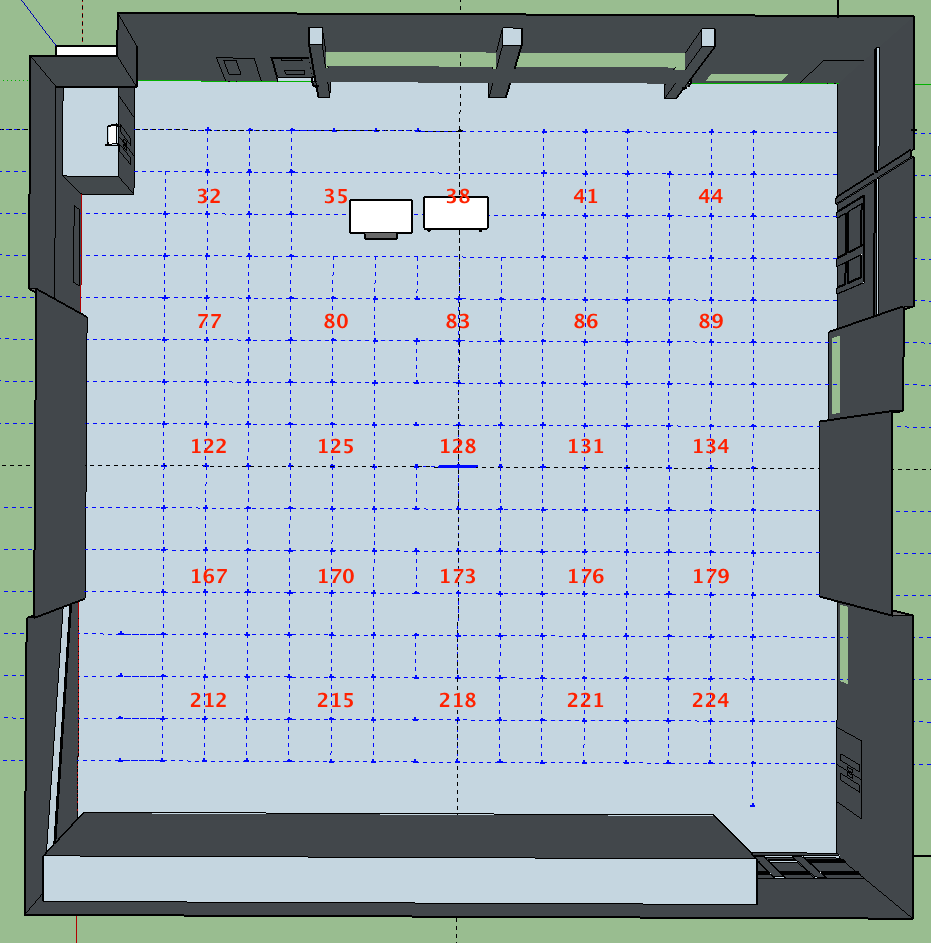
\includegraphics[scale = 0.23]{Sections/Appendix/AppendixA/images/Odeon/3m.png}}
				\caption{\ac{RIR} grid with 3m separation}
				\label{3m}
		\end{figure}
		\end{minipage}

			\begin{minipage}{0.5\textwidth}
		\begin{figure}[H]
				\centerline{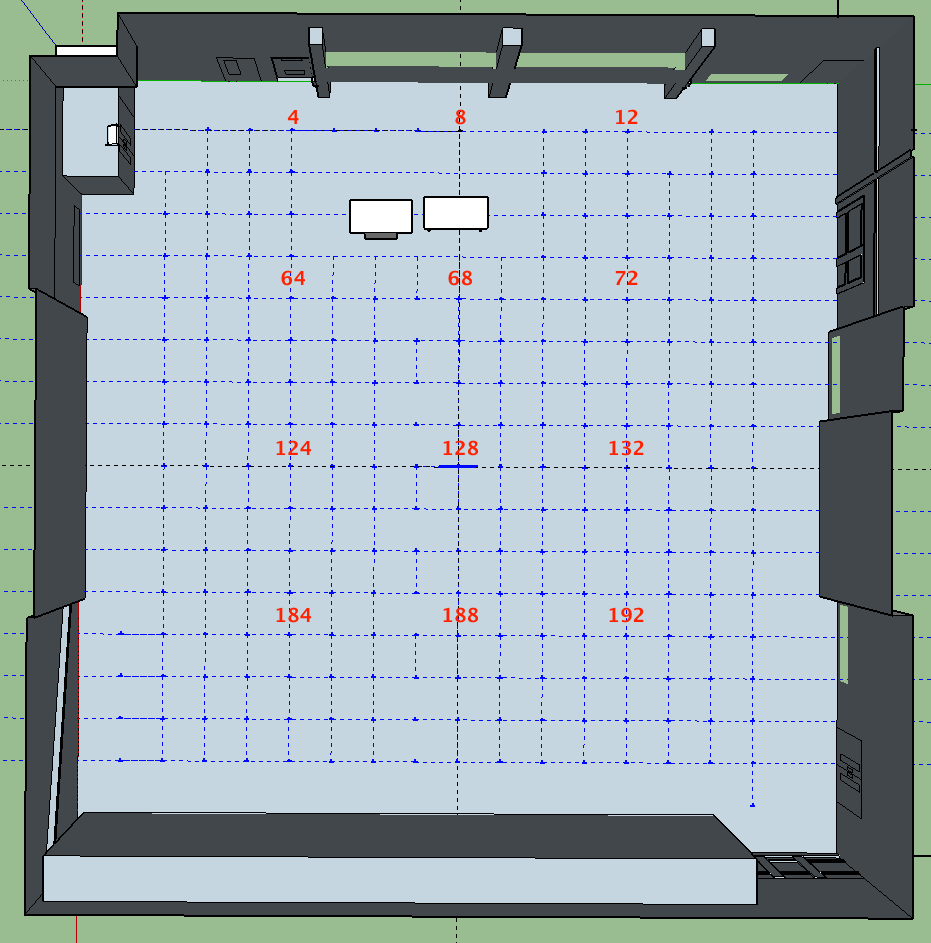
\includegraphics[scale = 0.23]{Sections/Appendix/AppendixA/images/Odeon/4m.png}}
				\caption{\ac{RIR} grid with 4m separation}
				\label{4m}
		\end{figure}
		\end{minipage}
		\begin{minipage}{0.5\textwidth}
		\begin{figure}[H]
				\centerline{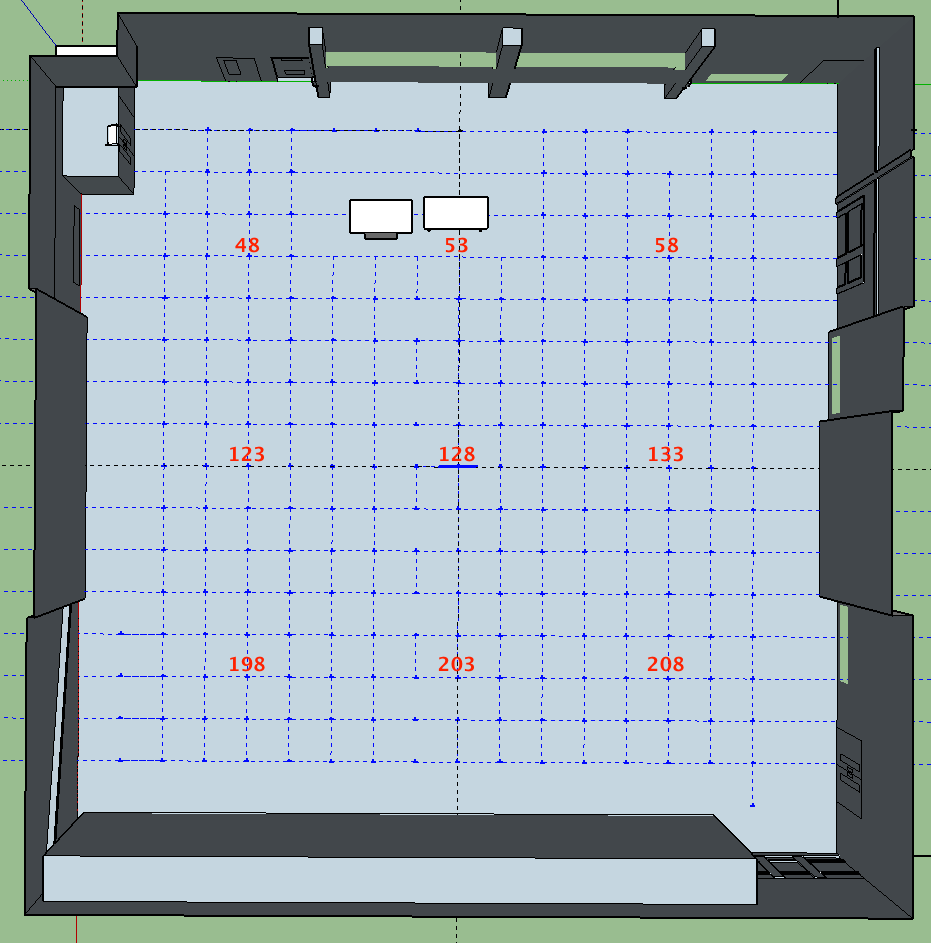
\includegraphics[scale = 0.23]{Sections/Appendix/AppendixA/images/Odeon/5m.png}}
				\caption{\ac{RIR} grid with 5m separation}
				\label{5m}
		\end{figure}
		\end{minipage}


	%-------------MAX APPENDIX-------------%
	\section{Appendix C}
	\label{appendixC}

		%-------------Panning Image-------------%
		\begin{figure}[H]
			\centerline{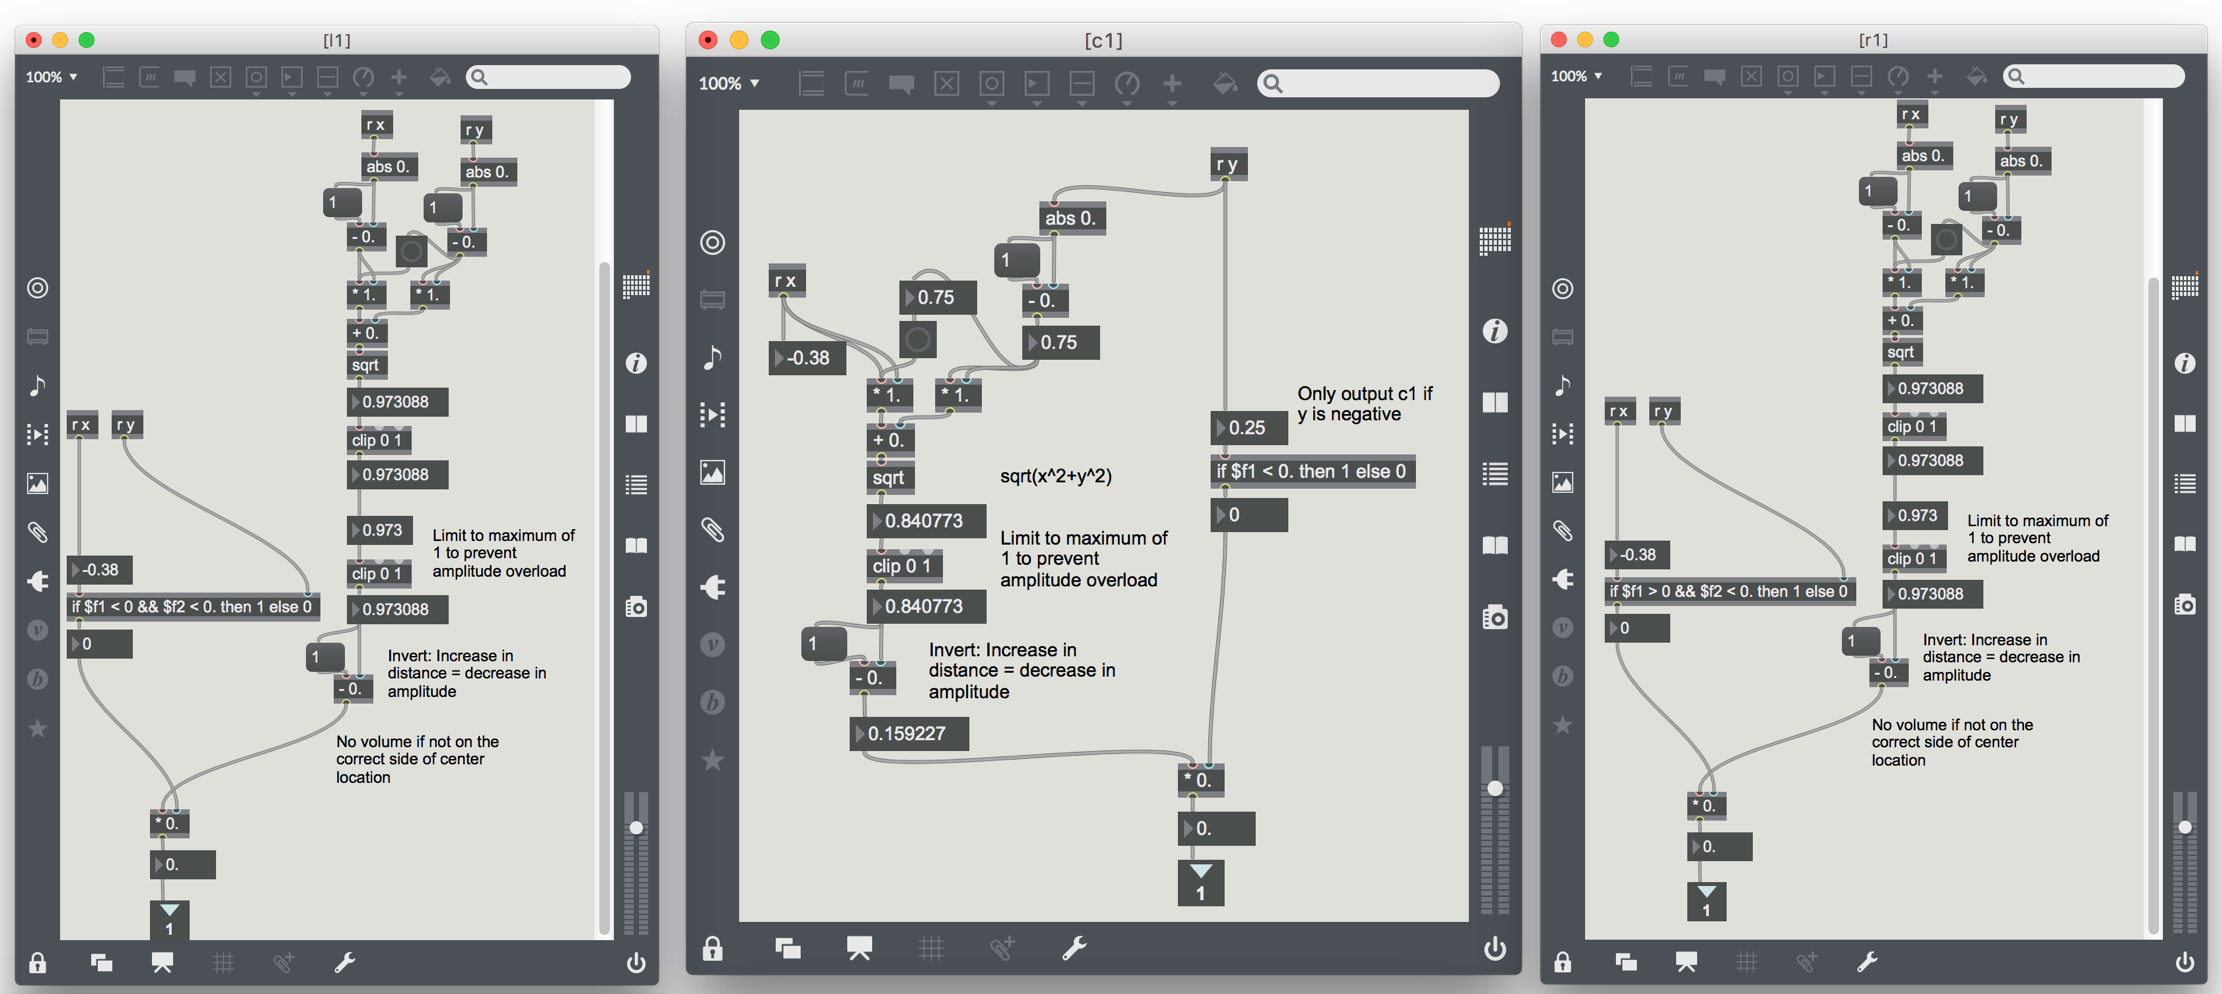
\includegraphics[scale = 0.4]{Sections/Implementation/Max/images/Max/iteration1/panning1.png}}
			\centerline{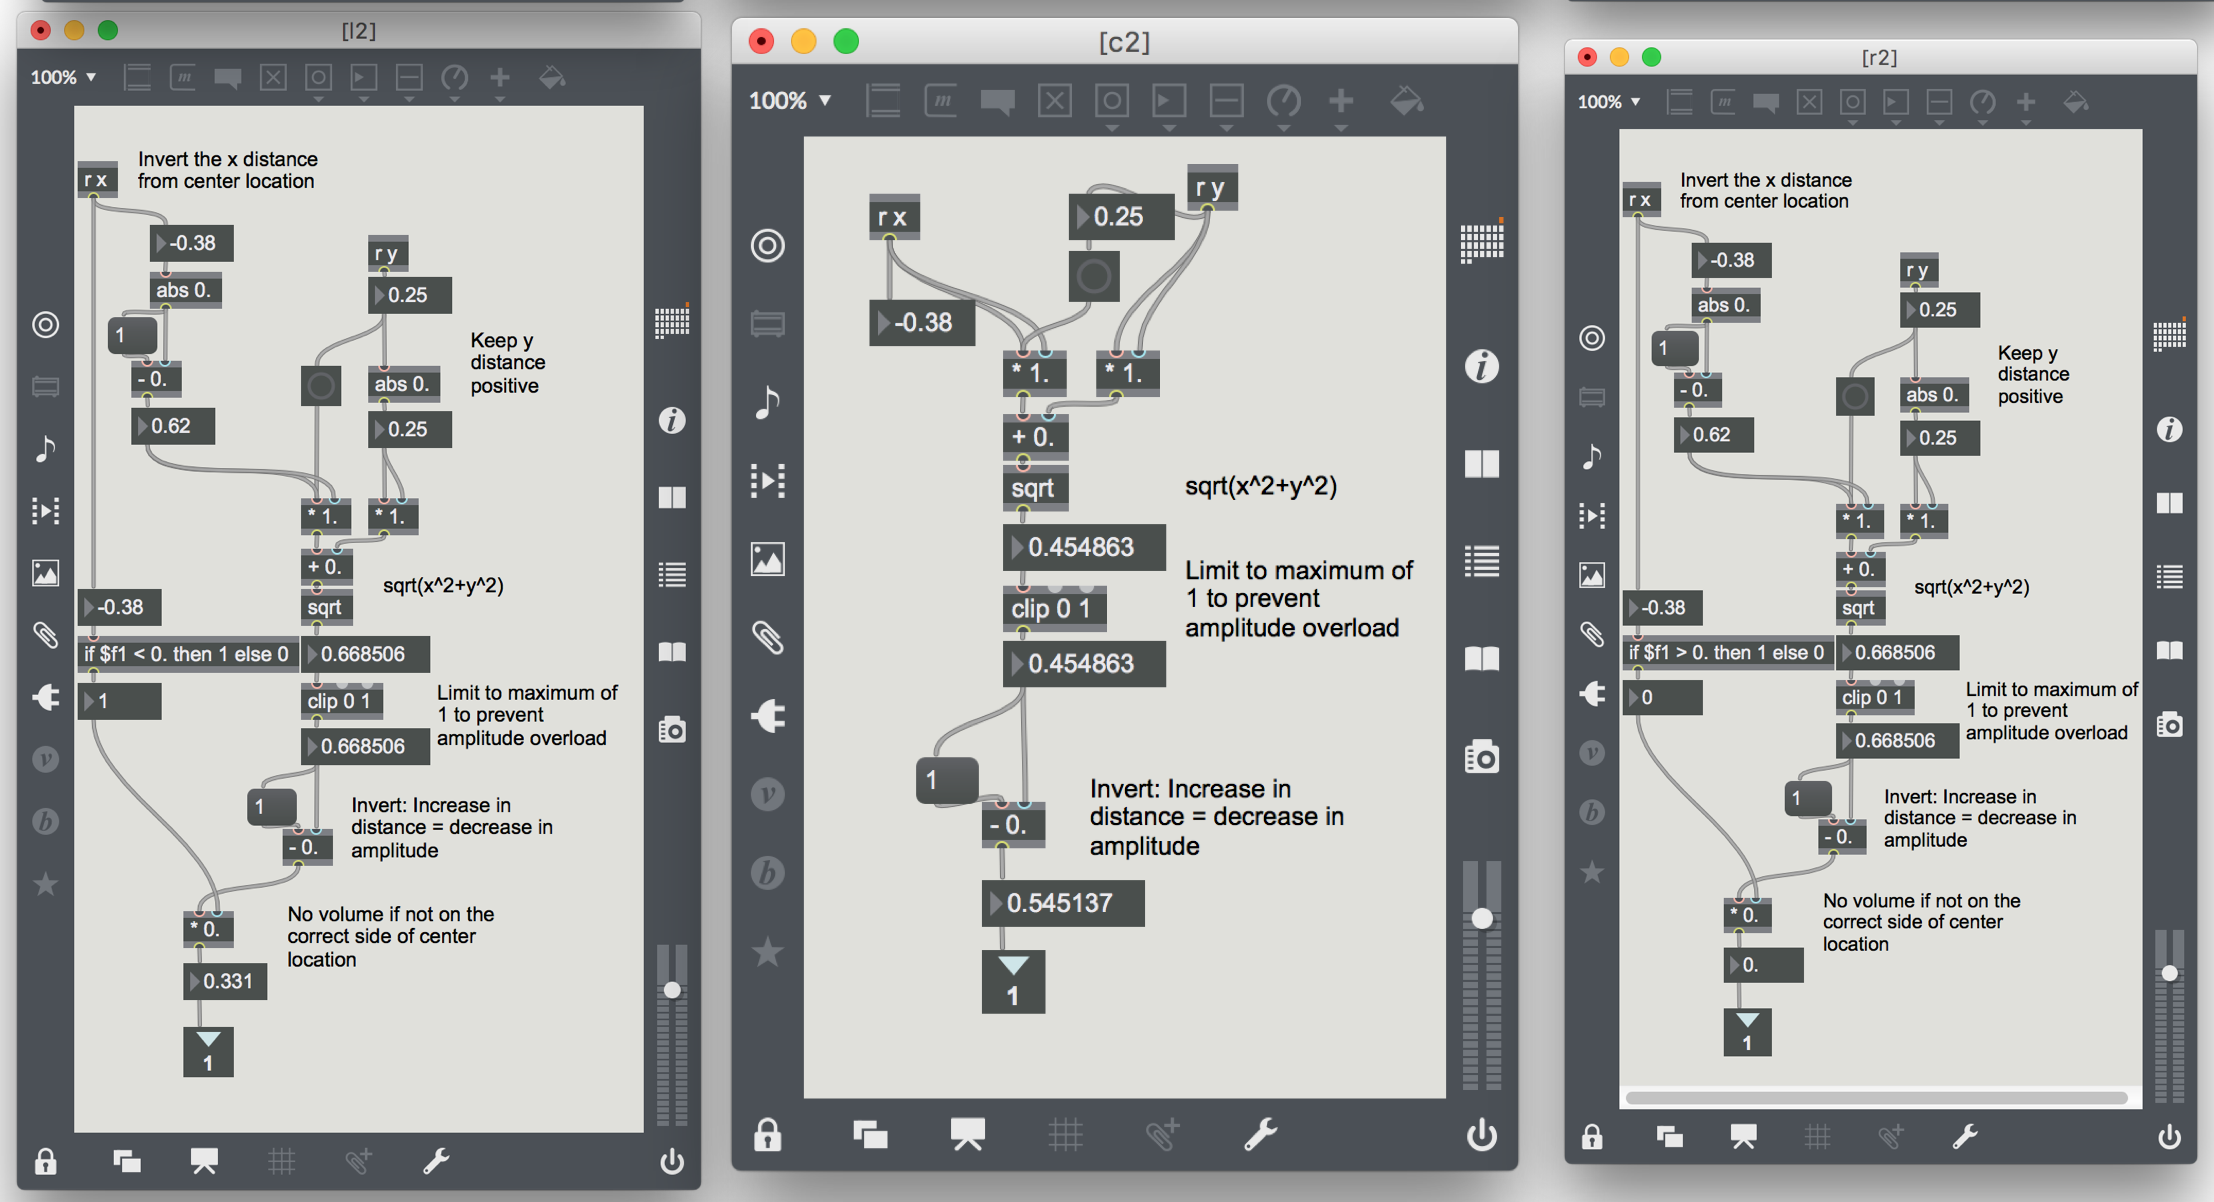
\includegraphics[scale = 0.4]{Sections/Implementation/Max/images/Max/iteration1/panning2.png}}
			\centerline{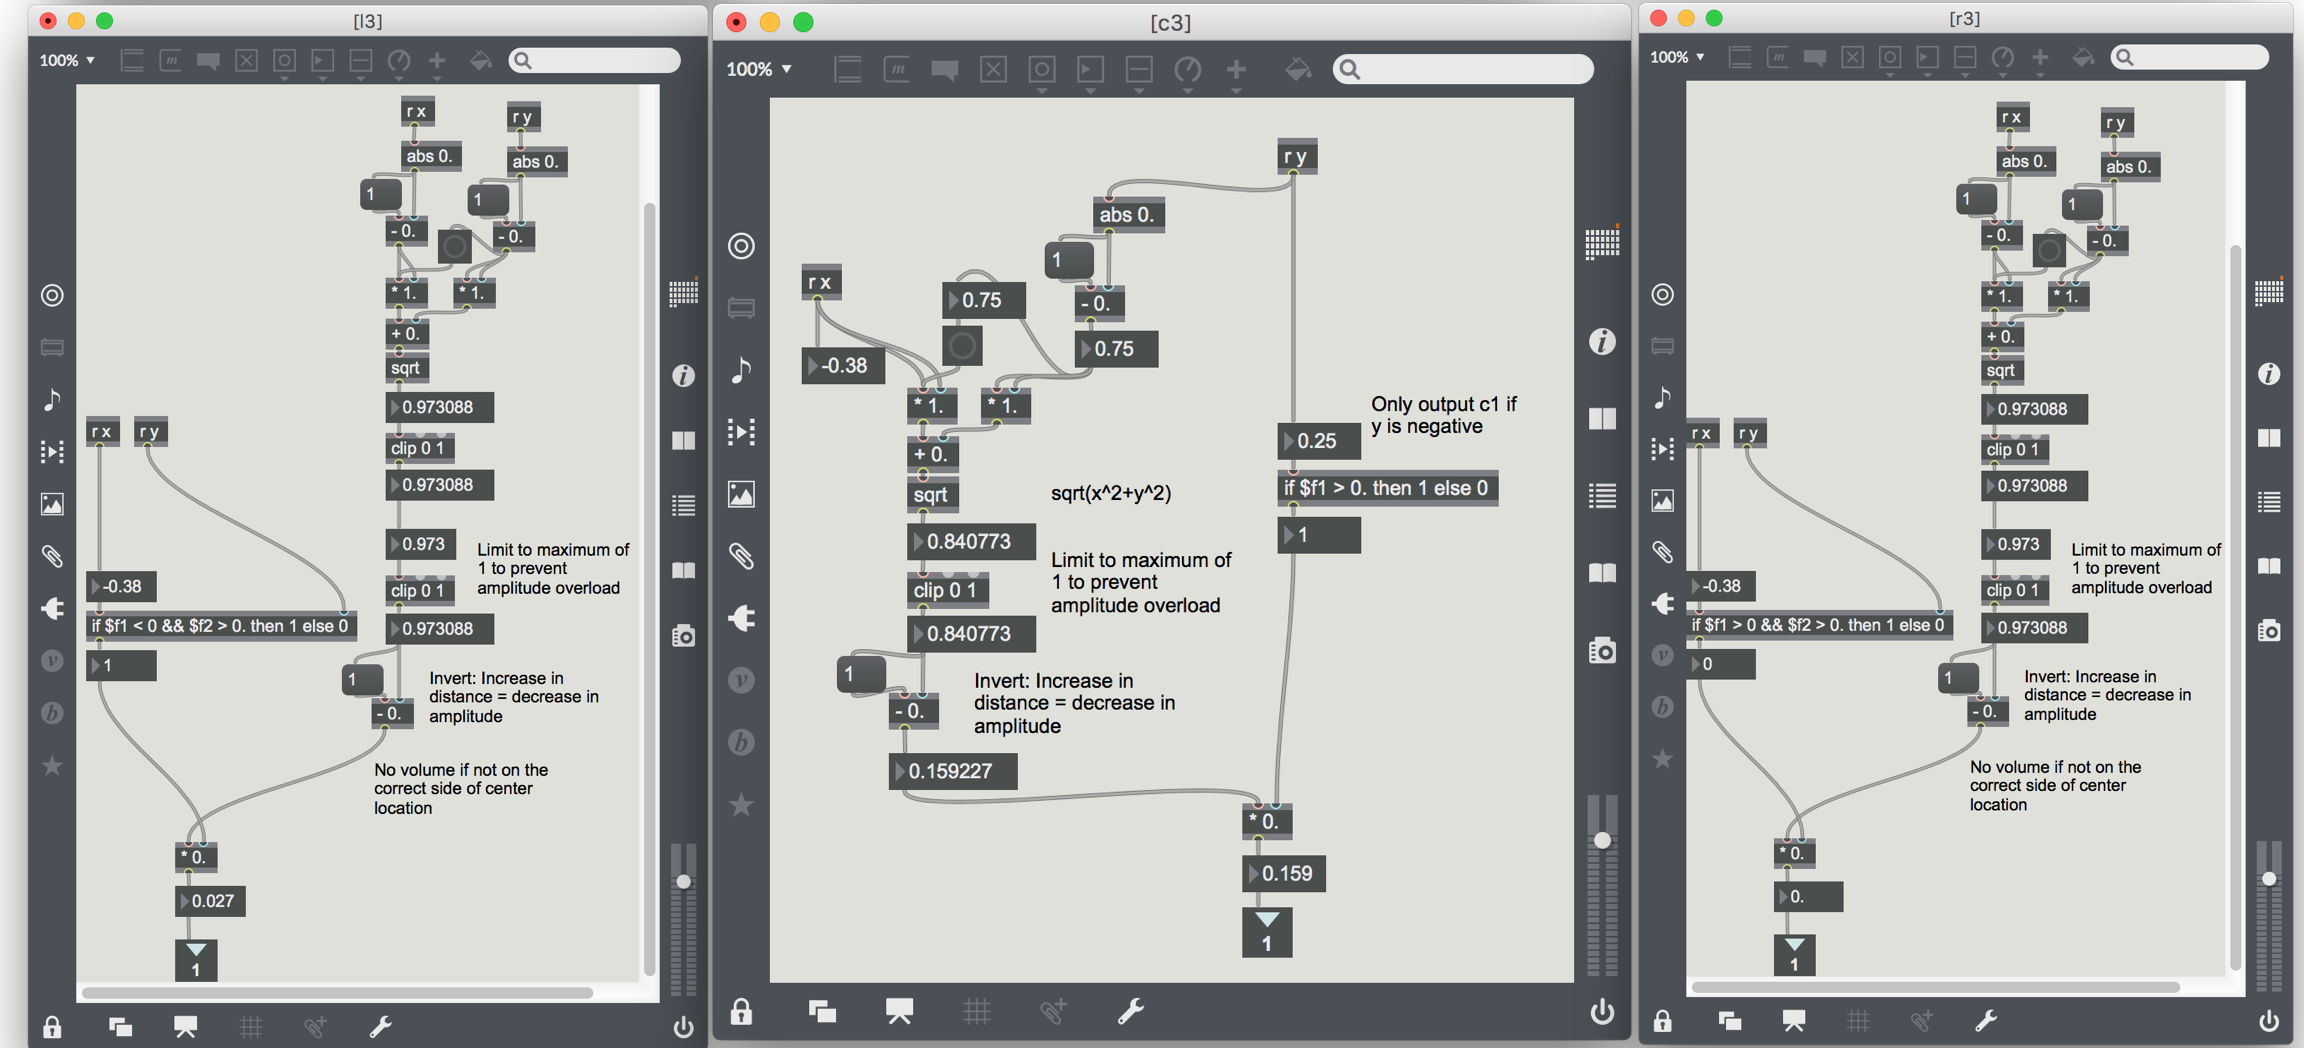
\includegraphics[scale = 0.4]{Sections/Implementation/Max/images/Max/iteration1/panning3.png}}
			\caption{Overview of the individual panning algorithms used in iteration 1.}
			\label{iteration1PanningCombined}
		\end{figure}

	\lstinputlisting[breaklines]{Sections/Appendix/AppendixA/Code/loadFilesLogic.js}

\end{appendices}

% \begin{figure}[ht]
% 			\center\includegraphics[scale =]{}
% 			\caption{}
% 			\label{}
% 		\end{figure}